%%%%%%%%%%%%%%%%%%%%%%%%%
% Dokumentinformationen %
%%%%%%%%%%%%%%%%%%%%%%%%%
\newcommand{\titleinfo}{Mobilkommunikation 1 - Formelsammlung}
\newcommand{\authorinfo}{F. Braun, L. Schmid, U. Giger, R. Koller} % Do not remove any names! Initial authors stay first.
\newcommand{\versioninfo}{$Revision: 1405 $ - powered by \LaTeX}
%%%%%%%%%%%%%%%%%%%%%%%%%%%%%%%%%%%%%%%%%%%%%
% Standard projektübergreifender Header für
% - Makros 
% - Farben
% - Mathematische Operatoren 
%
% DORT NUR ERGÄNZEN, NICHTS LÖSCHEN
%%%%%%%%%%%%%%%%%%%%%%%%%%%%%%%%%%%%%%%%%%%%%  
% Genereller Header
\documentclass[10pt,twoside,a4paper,fleqn]{article}
\usepackage[utf8]{inputenc}
\usepackage[left=1cm,right=1cm,top=1cm,bottom=1cm,includeheadfoot]{geometry}
\usepackage[ngerman]{babel,varioref}

% Pakete
\usepackage{amssymb,amsmath,fancybox,graphicx,color,lastpage,wrapfig,fancyhdr,hyperref,verbatim,floatflt}


%%%%%%%%%%%%%%%%%%%%
% Generelle Makros %
%%%%%%%%%%%%%%%%%%%%
\newcommand{\formelbuch}[1]{\footnotesize{(Skript S. #1)}\normalsize{}}
\newcommand{\verweis}[2]{\small{(siehe auch \ref{#1}, #2 (S. \pageref{#1}))}}
\newcommand{\subsubadd}[1]{\textcolor{black}{\mbox{#1}}}
\newcommand{\todo}[1]{\textcolor{red}{\textbf{\textit{TODO: #1}}}}

\newcommand{\matlab}[1]{\footnotesize{(Matlab: \texttt{#1})}\normalsize{}}


\newenvironment{liste}[0]{
	\begin{list}{$\bullet$}{\setlength{\itemsep}{0cm}\setlength{\parsep}{0cm} \setlength{\topsep}{0cm}}}
    {\end{list}}
\newenvironment{aufzaehlung}[0]{
	\begin{enumerate}{\setlength{\itemsep}{0cm}\setlength{\parsep}{0cm}
	\setlength{\topsep}{0cm}}} {\end{enumerate}}    

\newcommand{\abbHeight}[3]{
	\begin{center}
		\includegraphics[height=#2]{./bilder/#1} \\
		#3
    \end{center}
}

%%%%%%%%%%
% Farben %
%%%%%%%%%%
\definecolor{black}{rgb}{0,0,0}
\definecolor{red}{rgb}{1,0,0}
\definecolor{white}{rgb}{1,1,1}
\definecolor{grey}{rgb}{0.8,0.8,0.8}
\definecolor{darkgrey}{rgb}{0.4,0.4,0.4}
\definecolor{orange}{rgb}{0.98,0.5,0.03}

%%%%%%%%%%%%%%%%%%%%%%%%%%%%
% Mathematische Operatoren %
%%%%%%%%%%%%%%%%%%%%%%%%%%%%
\DeclareMathOperator{\sinc}{sinc}



% Fouriertransformationen
\unitlength1cm
\newcommand{\FT}
{
\begin{picture}(1,0.5)
\put(0.2,0.1){\circle{0.14}}\put(0.27,0.1){\line(1,0){0.5}}\put(0.77,0.1){\circle*{0.14}}
\end{picture}
}


\newcommand{\IFT}
{
\begin{picture}(1,0.5)
\put(0.2,0.1){\circle*{0.14}}\put(0.27,0.1){\line(1,0){0.45}}\put(0.77,0.1){\circle{0.14}}
\end{picture}
}



%%%%%%%%%%%%%%%%%%%%%%%%%%%%
% Allgemeine Einstellungen %
%%%%%%%%%%%%%%%%%%%%%%%%%%%%
%pdf info
\hypersetup{pdfauthor={\authorinfo},pdftitle={\titleinfo},colorlinks=false}
\author{\authorinfo}
\title{\titleinfo}

%Kopf- und Fusszeile
\pagestyle{fancy}
\fancyhf{}
%Linien oben und unten
\renewcommand{\headrulewidth}{0.5pt} 
\renewcommand{\footrulewidth}{0.5pt}

\fancyhead[L]{\titleinfo{ }\tiny{(\versioninfo)}}
%Kopfzeile rechts bzw. aussen
\fancyhead[R]{Seite \thepage { }von \pageref{LastPage}}
%Fusszeile links bzw. innen
\fancyfoot[L]{\footnotesize{\authorinfo}}
%Fusszeile rechts bzw. ausen
\fancyfoot[R]{\footnotesize{\today}}

% Einrücken verhindern versuchen
\setlength{\parindent}{0pt}



% Möglichst keine Ergänzungen hier, sondern in header.tex
\begin{document} 
\section{Logarithmische Darstellungen}

\begin{tabular}{ll}
\parbox{7cm}{ 
    \scriptsize
    \renewcommand{\arraystretch}{1.2}
    \begin{tabular}{|c|c|c|c|}
    \hline
    \textbf{Lrel. (dB)} & \textbf{Lrel. (NP)} & \textbf{P2/P1} & \textbf{A2/A1} \\ \hline
    $100.000$ & $11.513$ & $10^{10}$ & $10^5$ \\ \hline
    $90.000$ & $10.362$ & $10^9$ & $31622.777$ \\ \hline
    $80.000$ & $9.210$ & $10^8$ & $10^4$ \\ \hline
    $70.000$ & $8.059$ & $10^7$ & $3162.278$ \\ \hline
    $60.000$ & $6.908$ & $10^6$ & $10^3$ \\ \hline
    $50.000$ & $5.756$ & $10^5$ & $316.228$ \\ \hline
    $40.000$ & $4.605$ & $10^4$ & $10^2$ \\ \hline
    $30.000$ & $3.454$ & $10^3$ & $31.623$ \\ \hline
    \textbf{$20.000$} & $2.303$ & \textbf{$10^2$} & \textbf{$10.000$} \\ \hline
    $19.085$ & $2.197$ & $81.000$ & $9.000$ \\ \hline
    $19.000$ & $2.187$ & $79.433$ & $8.913$ \\ \hline
    $18.062$ & $2.079$ & $64.000$ & $8.000$ \\ \hline
    $18.000$ & $2.072$ & $63.096$ & $7.943$ \\ \hline
    $17.000$ & $1.957$ & $50.119$ & $7.079$ \\ \hline
    $16.902$ & $1.946$ & $49.000$ & $7.000$ \\ \hline
    $16.000$ & $1.842$ & $39.811$ & $6.310$ \\ \hline
    $15.563$ & $1.792$ & $36.000$ & $6.000$ \\ \hline
    $15.000$ & $1.727$ & $31.623$ & $5.623$ \\ \hline
    $14.000$ & $1.612$ & $25.119$ & $5.012$ \\ \hline
    \textbf{$13.979$} & $1.609$ & \textbf{$25.000$} & \textbf{$5.000$} \\ \hline
    $13.000$ & $1.497$ & $19.953$ & $4.467$ \\ \hline
    \textbf{$12.041$} & $1.386$ & \textbf{$16.000$} & \textbf{$4.000$} \\ \hline
    \textbf{$12.000$} & $1.382$ & $15.849$ & $3.981$ \\ \hline
    $11.000$ & $1.266$ & $12.589$ & $3.548$ \\ \hline
    \textbf{$10.000$} & $1.151$ & \textbf{$10.000$} & $3.162$ \\ \hline
    $9.542$ & $1.099$ & $9.000$ & $3.000$ \\ \hline
    $9.000$ & $1.036$ & $7.943$ & $2.818$ \\ \hline
    $8.000$ & $0.921$ & $6.310$ & $2.512$ \\ \hline
    $7.000$ & $0.806$ & $5.012$ & $2.239$ \\ \hline
    \textbf{$6.021$} & \textbf{$0.693$} & \textbf{$4.000$} & \textbf{$2.000$} \\ \hline
    $6.000$ & $0.691$ & $3.981$ & $1.995$ \\ \hline
    $5.000$ & $0.576$ & $3.162$ & $1.778$ \\ \hline
    $4.000$ & $0.461$ & $2.512$ & $1.585$ \\ \hline
    \textbf{$3.010$} & \textbf{$0.347$} & \textbf{$2.000$} & \textbf{$1.414$} \\ \hline
    $3.000$ & $0.345$ & $1.995$ & $1.413$ \\ \hline
    $2.000$ & $0.230$ & $1.585$ & $1.259$ \\ \hline
    $1.000$ & $0.115$ & $1.259$ & $1.122$ \\ \hline
    $0.000$ & $0.000$ & $1.000$ & $1.000$ \\ \hline
    -$1.000$ & -$0.115$ & $0.794$ & $0.891$ \\ \hline
    -$2.000$ & -$0.230$ & $0.631$ & $0.794$ \\ \hline
    -$3.000$ & -$0.345$ & $0.501$ & $0.708$ \\ \hline
    -$4.000$ & -$0.461$ & $0.398$ & $0.631$ \\ \hline
    -$5.000$ & -$0.576$ & $0.316$ & $0.562$ \\ \hline
    -$6.000$ & -$0.691$ & $0.251$ & $0.501$ \\ \hline
    -$7.000$ & -$0.806$ & $0.200$ & $0.447$ \\ \hline
    -$8.000$ & -$0.921$ & $0.158$ & $0.398$ \\ \hline
    -$9.000$ & -$1.036$ & $0.126$ & $0.355$ \\ \hline
    -$10.000$ & -$1.151$ & $0.100$ & $0.316$ \\ \hline
    -$15.000$ & -$1.727$ & $0.032$ & $0.178$ \\ \hline
    -$20.000$ & -$2.303$ & $10^{-2}$ & $0.100$ \\ \hline
    -$30.000$ & -$3.454$ & $10^{-3}$ & $0.032$ \\ \hline
    -$40.000$ & -$4.605$ & $10^{-4}$ & $0.010$ \\ \hline
    -$50.000$ & -$5.756$ & $10^{-5}$ & $0.003$ \\ \hline
    -$60.000$ & -$6.908$ & $10^{-6}$ & $0.001$ \\ \hline
    -$70.000$ & -$8.059$ & $10^{-7}$ & $0.000$ \\ \hline
    -$80.000$ & -$9.210$ & $10^{-8}$ & $10^{-4}$ \\ \hline
    -$90.000$ & -$10.362$ & $10^{-9}$ & $3.162 \cdot 10^{-5}$ \\ \hline
    -$100.000$ & -$11.513$ & $10^{-10}$ & $10^{-5}$ \\ \hline
    \end{tabular}
    \renewcommand{\arraystretch}{1.0}

    \normalsize
}
& \parbox{11.5cm}{
Verstärkungsmass L in \textbf{Dezibel} (dB):\\
$L_P = 10 \cdot \log \left(\frac {P_2} {P_1}\right)$ \\
$L_A = 20 \cdot \log \left(\frac {A_2} {A_1}\right)$ \\ 

Dezibel L zu linear: \\
$P_2 = P_1 \cdot 10^{\frac{L_P}{10}} $ \\
$A_2 = A_1 \cdot 10^{\frac{L_A}{20}} $ \\

Verstärkungsmass L in \textbf{Neper} (Np):\\
$L_P = \frac {1}{2} \cdot \ln \left(\frac {P_2} {P_1}\right)$\\
$L_A = \ln \left(\frac {A_2} {A_1} \right)$ \\

Neper zu linear: \\
$P_2 = P_1 \cdot e^{2 L_P}$ \\
$A_2 = A_1 \cdot e^{L_A}$ \\

Die Umrechnung zwischen {\bf dB} und {\bf Np} ist linear: \\
$1\mbox{~dB} = \frac {\ln(10)} {20} \mbox{~Np} = 0.1151\mbox{~Np}$ \\
$1\mbox{~Np} = 20 \cdot \log(\mbox{e}) \mbox{~dB} = 8.686\mbox{~dB}$ \\ 
\\
Anstatt $\frac{X_2}{X_1}$ für Verstärkungsmasse ($L$) können auch
$\frac{X_1}{X_2}$ für Dämpfungsmasse ($a$) verwendet werden!

\small{($P$ für Leistungen, $A$ für Amplituden)}
\\ \\ \\

\textbf{Hilfen zur Berechnung}\\
\begin{tabular}{|l|ll|}
\hline
$x Db$  & $L_P=P_2/P_1$ &$L_A=A_2/A_1$ \\
\hline
$-x dB$ & $1/L_P$   & $1/L_A$\\
$x+3dB$ & $L_P \cdot 2$ & $L_A \cdot \sqrt{2} \approx L_A \cdot 1.414$ \\
$x+10dB$    & $L_P \cdot 10$ & $L_A \cdot \sqrt{10} \approx L_A \cdot 3.162$\\
\hline
\end{tabular}
\\ \\ \\

\textbf{Relative \& absolute Pegel}\\
Relativer Pegel: Pegel relativ zu definiertem Wert\\
Absoluter Pegel: Pegel an Normgenerator ($R_i = 600 \Omega$, $1mW$ Leistung am
Widerstand)\\ 
\begin{tabular}{|l|l|l|}\hline
  & dBu & Spannungspegel bezogen auf 774.6~mV an 600~$\Omega$\\ \cline{2-3}
 \multicolumn{1}{|l|}{\raisebox{1.5ex}[-1.5ex]{$\mbox{dB}_{abs.}$}} & dBm & Leistungspegel bezogen auf 1~mW an 600~$\Omega$\\ \hline\hline
  & dBV & Spannungspegel bezogen auf 1~V\\ \cline{2-3}
  & dB$\mu$V & Spannungspegel bezogen auf 1~$\mu$V\\ \cline{2-3}
  & dBf & Leistungspegel bezogen auf $10^{-15}$~W\\ \cline{2-3} 
\multicolumn{1}{|l|}{$\mbox{dB}_{rel.}$}  & dBW & Leistungspegel bezogen auf 1~W\\ \cline{2-3}
  & dBk & Leistungspegel bezogen auf 1~kW\\ \cline{2-3}
  & dBr & relativer Pegel\\ \cline{2-3}
  & dB0 & Pegel auf 0~dB bezogen\\ \hline
\end{tabular}\\ \\ \\
\textbf{Addition von Pegeln} \\
dB $\pm$ dB = dB \\ 
dBm $\pm$ dB = dBm \\ 
dBm - dBm = dB \\
dBm + dBm : nicht direkt möglich $\Rightarrow$ siehe Anhang A.2.3
\formelbuch{280} }
\end{tabular}
\newpage

\section{HF-Design}
\subsection{Parasitäre Effekte \formelbuch{9}}
Selbstimpedanz einer Leitung: $ L=0.002 l \left(\ln\left(\frac {4l}d-0.75
\right) \right) \text{[$\mu$H]}$

\subsection{Impedanzanpassung \formelbuch{10}}
\begin{tabular}{lll}
\parbox{10cm}{
	Impedanzanpassung der Last durch konjugiert komplexe Quellenimpedanz.\\
	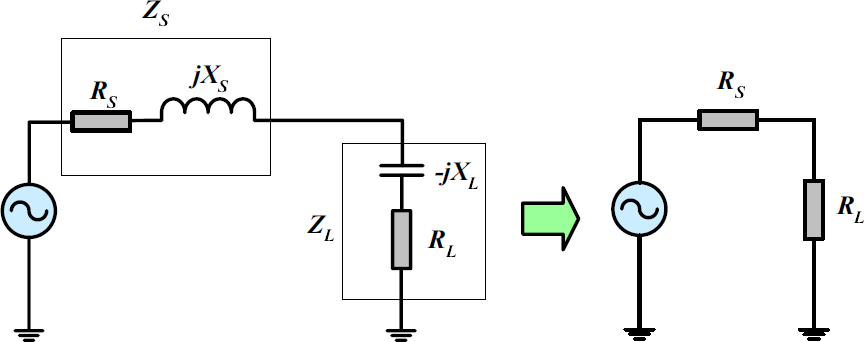
\includegraphics[height=2cm]{./bilder/rfdesign_matching.png}
    }
& \parbox{3cm}{
    L-Netzwerk.\\
    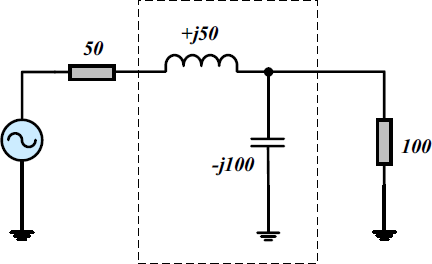
\includegraphics[height=2cm]{./bilder/rfdesign_matching_L_network.png}
    }
& \parbox{3cm}{
    $\pi$-Netzwerk.\\
    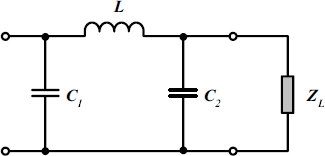
\includegraphics[height=2cm]{./bilder/rfdesign_matching_pi_network.png}
    }
\end{tabular}\\

\subsection{S-Parameter \formelbuch{13}}
\begin{tabular}{lll}
        $S = \begin{bmatrix} s_{11} & s_{12} \\ s_{21} & s_{22} 
         \end{bmatrix}$
    & \parbox{8cm}{
        $s_{11} = \left . \frac{ b_1}{ a_1} \right|_{ a_2=0} 
                         = \text{input reflection coefficient}$ \\
        $s_{21} = \left . \frac{ b_2}{ a_1} \right|_{ a_2=0} 
                         = \text{forward gain}$ \\
        $s_{12} = \left . \frac{ b_1}{ a_2} \right|_{ a_1=0} 
                         = \text{backward gain}$ \\
        $s_{22} = \left . \frac{ b_2}{ a_2} \right|_{ a_1=0} 
                         = \text{output reflection coefficient}$ \\ \\
        }
    & \parbox{7cm}{
        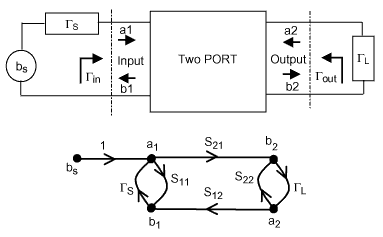
\includegraphics[width=6.5cm]{./bilder/rfdesign_s-parameter.png}
        }\\
\end{tabular}

\subsubsection{Eigenschaften der S-Parameter }
\begin{tabular}{|l|l|}
\hline
Reziprozität
    & $s_{21} = s_{12}$, passive Netzwerke erfüllen dies \\
\hline
Symmetrie
    & Zusätzlich zur Reziprozität ist $s_{11} = s_{22}$ \\
\hline
Verlustlos
    & $| s_{11}|^2 +  | s_{21}|^2 = 1 \cap | s_{22}|^2 +  |
    s_{12}|^2 = 1 \cap s_{11}^*  s_{12} +  s_{21}^*  s_{22} = 0$ \\
\hline
Simultaneous Conjugate Match
    & $(\Gamma_{in} = -\Gamma_L = \Gamma_S^* \quad \bigcap \quad 
    \Gamma_{out} = -\Gamma_S = \Gamma_L^*) \Rightarrow \Gamma_S = - \Gamma_L^*$
    \\
\hline
\hline
Reflexionskoeffizienten
    & $\Gamma_x = r_x$ \\
\hline
Reflexion
    & $\Gamma_{\text{in}} = 
    s_{11} + \frac{s_{12}s_{21}\Gamma_{\text{L}}}{1-s_{22}\Gamma_{\text{L}}}$ \\
\hline
Reflexionsdämpfung (Return Loss)
    & $\text{RL}=
    \frac{\text{forwarded power}}{\text{reflected power}} \text{ [dB]} =
    -20\log_{10} |\Gamma| \underbrace{=}_{\text{passiv, verlustfrei}} -10
    \log_{10}(1-|s_{21}|)$\\
\hline
Einfügedämpfung (Insertion Loss)
    & $\text{IL}= -20 \log_{10}(|s_{21}|) = -10
    \log_{10}(\frac{P_{R_L}}{P_{tot}})$ \\
\hline
Stehwellenverhältnis (Standing Wave Ratio)
    & $ \text{VSWR} = \dfrac{U_{\text{max}}}{U_{\text{min}}} $ \\
\hline
Güte
    & $Q = \dfrac{|\operatorname{Im}(Z)|}{|\operatorname{Re}(Z)|} =
    \dfrac{|X|}{R}$ \\
\hline
Isolation
    & $isolation = - 20 \log_{10} s_{12} = [dB]$\\
\hline
Richtwirkung
    & $directivity = isolation - 20 \log_{10} s_{21} = [dB]$ \\
\hline
\end{tabular}

\subsubsection{Umwandlung von Verlustparametern}
\textcolor{red}{gültig für
$|\Gamma\le 1|$} / \textcolor{blue}{gültig für reale (positive) Impedanzen}\\
\begin{tabular}{|r|l|l|l|l|}
\hline
     & $f(Z)$ & $f(\Gamma)$ 
              & $f(\text{VSWR})$ 
              & $f(\text{RL} \text{\,[dB]})$ \\  \hline \hline 

$Z=$ & ---    & $\frac{1+\Gamma}{1-\Gamma}Z_0$
              & \textcolor{red}{---} /
                \textcolor{blue}{$\text{VSWR}^{\pm 1}\cdot Z_0$}
              & \textcolor{red}{---} /
                \textcolor{blue}{$\frac{1+10^{-\text{RL}/20}}{1-10^{-\text{RL}/20}}^{\pm 1}\cdot Z_0$} \\ 
\hline 
$\Gamma=$ & \textcolor{red}{$\frac{Z-Z_0}{Z+Z_0}$} /
                \textcolor{blue}{$\frac{R-Z_0}{R+Z_0}$ }
                 & --- 
                 &
                 \textcolor{red}{$|\Gamma|=\frac{\text{VSWR}-1}{\text{VSWR}+1}$} /
                \textcolor{blue}{$\pm \frac{\text{VSWR}-1}{\text{VSWR}+1}$}
                 & \textcolor{red}{$|\Gamma|= 10^{-\text{RL}/20}$} /
                \textcolor{blue}{$\pm 10^{-\text{RL}/20}$} \\ 
\hline
$\text{VSWR}=$& \textcolor{red}{$\frac{1+\left|\frac{Z-Z_0}{Z+Z_0} \right|}%
                      {1-\left|\frac{Z-Z_0}{Z+Z_0} \right|}$} /
                \textcolor{blue}{$\max\left(\frac R{Z_0},\frac{Z_0}R \right)$}
              & $\frac{1+|\Gamma|}{1-|\Gamma|}$
              & ---
              & $\frac{1+10^{-\text{RL}/20}}{1-10^{-\text{RL}/20}}$ \\ 
\hline
$\text{RL}=$  & \textcolor{red}{$20\log_{10}\left|\frac{Z+Z_0}{Z-Z_0} \right|$}
/
                \textcolor{blue}{$20\log_{10}\left|\frac{R+Z_0}{R-Z_0} \right|$}
              & $-20\log_{10}\left|\Gamma \right|$
              & $20\log_{10}\left(\frac{\text{VSWR}+1}{\text{VSWR}-1} \right)$
                & --- \\ 
\hline
\end{tabular}

\subsubsection{Kaskade zweier Zeitore \formelbuch{15}}
1. In T-Matrix: $T = \frac 1{s_{21}} 
  \begin{bmatrix} -\det S & s_{11} \\ -s_{22} & 1 \end{bmatrix}$ \qquad 
2. Matrixmultiplikation $T_1 \cdot T_2$ \qquad 3. In S-Matrix: $S = \frac
1{t_{22}} \begin{bmatrix} t_{12} & \det T  \\ 1 & -t_{21} \end{bmatrix}$

\newpage
\subsection{Smith-Chart \formelbuch{18}}
\begin{tabular}{ll}
\parbox{9cm}{
	\textbf{Smith Chart und Richtungen der Schaltelemente}\\
	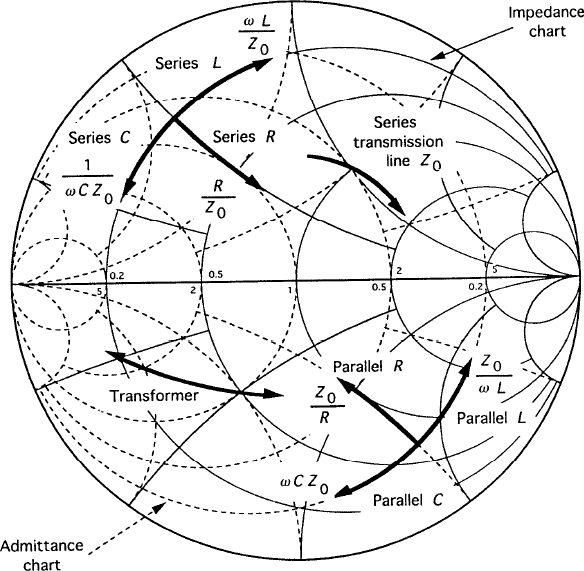
\includegraphics[width=8.5cm]{./bilder/rfdesign_smithchart_directions.png}
    }
& \parbox{9cm}{
    \textbf{$s_{11}$ für einige Elemente} \tiny{Pfeilspitze: HF - Pfeilanfang:
    DC}\\
    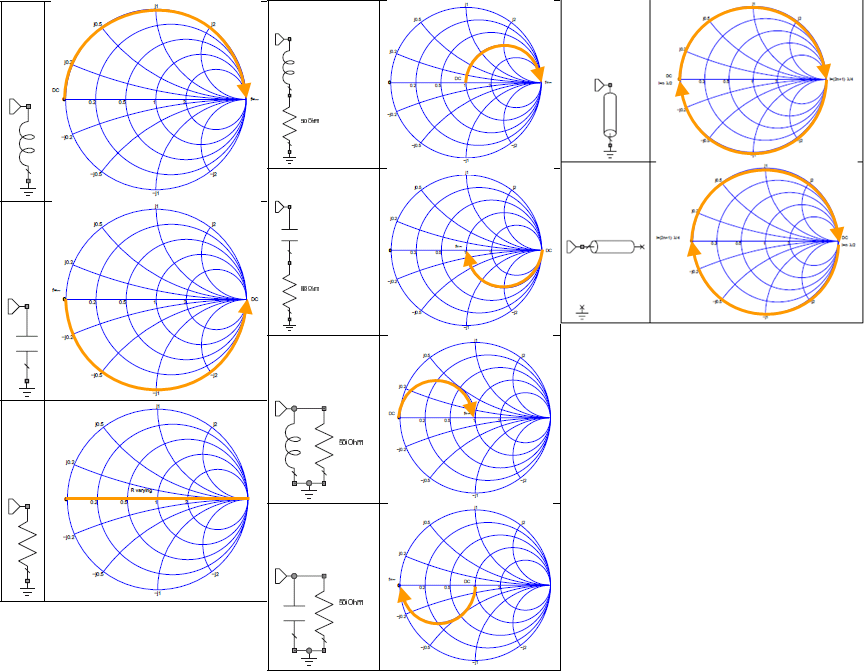
\includegraphics[width=8.5cm]{./bilder/rfdesign_smithchart_s11.png}
    } \\
\vspace{0.2cm}\\
\parbox{9cm}{
    \begin{liste}
      \item \textbf{Normieren:} $Z_{\text{einzutragen}} = \frac{Z}{Z_0}$
      \item \textbf{Impedanz $\Leftrightarrow$ Admittanz:} Am Kreismittelpunkt spiegeln
      \item \textbf{Kurzschluss:}   \textcolor{yellow}{Impedanz} \textcolor{orange}{Admittanz}
      \item \textbf{Leerlauf:}      \textcolor{orange}{Impedanz} \textcolor{yellow}{Admittanz}
      \item \textbf{Phase:} Verlängerung der Reflexionsgerade an Kreisrand und Winkel ablesen
      \item \textbf{SWR:} Kreis mit Radius $|\Gamma|$ auf reeller Achse
      \item \textbf{Leitungslänge:} Äusserste Skala am Kreisrand  $\frac{l}{\lambda}$
      \item \textbf{Entnormieren:} $Z_{\text{gewünscht}} = Z_0
      Z_{\text{abgelesen}}$
    \end{liste}
    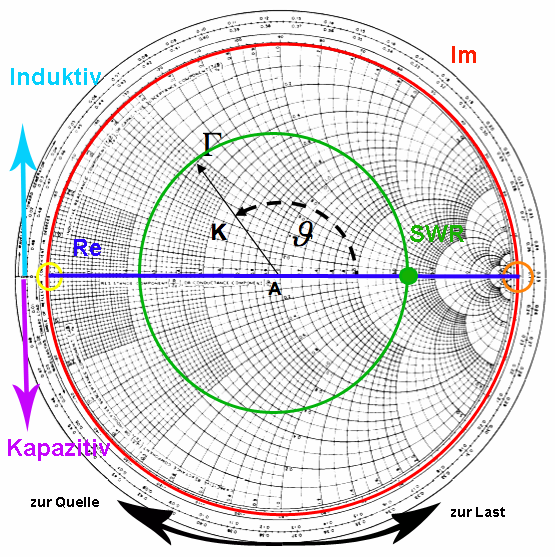
\includegraphics[height=7cm]{../Elt4/bilder/SmithChart2.png}
    }
& \parbox{9cm}{
    \textbf{Anpassungsnetzwerke} \\
    \small{Impedanzen innerhalb der nicht-schattierten Regionen sind in eine
    resistive Ladung $Z_0$ mit den gegebenen L-Netzwerken transformierbar}.
    Reine C Netzwerke gegenüber L oder L/C bevorzugt: Abkopplung des
    Bias-DC, günstiger, weniger Verluste. \\
    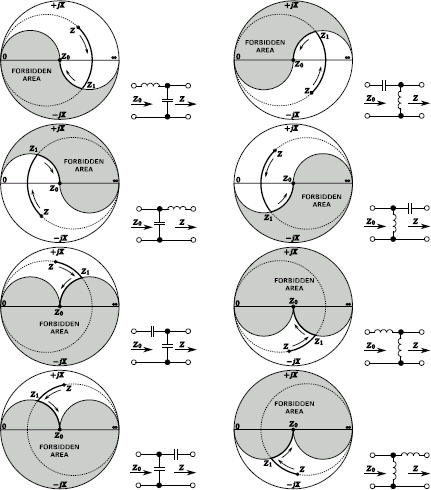
\includegraphics[width=8.5cm]{./bilder/rfdesign_smithchart_matching_Ltypes.png}
    }
\end{tabular}

\subsection{Skin Effekt \formelbuch{28}}
Je höher die Frequenz ist, desto eher fliesst der Strom nur noch an der
Leitungsoberfläche (Skintiefe). \\
\textbf{Skintiefe} $\delta = \sqrt{\frac{\lambda}{\pi\sigma\mu v}}
         = \sqrt{\frac{1}{\pi\sigma\mu f}}$ \qquad
\textbf{Stromdichte} $|J|=J_0 e^{-\frac x{\delta}}$ \qquad 
\textbf{Strom} $I = \int\limits_{0}^{\infty} J_0 e^{-\frac{x}{\delta}} dx = J_0
\delta$\\

\subsection{Leitungstheorie \formelbuch{32}}
\small
    \begin{tabular}{p{8cm}p{4cm}p{5.5cm}}
        \begin{minipage}{8cm}
            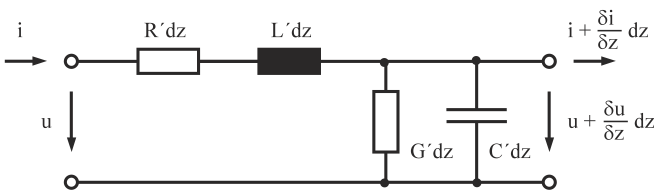
\includegraphics[width=8cm]{../Elt4/bilder/LeitungselementESB}
        \end{minipage}&
        \begin{minipage}{4.5cm}
            \textbf{Leitungsbeläge}\\
            $R'[\frac{\Omega}{m}]: \text{Widerstandsbelag}$\\
            $L'[\frac{H}{m}]: \text{Induktivitätsbelag}$\\
            $G'[\frac{S}{m}]: \text{Leitwertbelag}$\\
            $C'[\frac{F}{m}]: \text{Kapazitätsbelag}$\\
        \end{minipage}&
        \begin{minipage}{5cm}
            \textbf{Leerlauf}:\\
                $\underline{Y}_L=\frac{1}{\underline{Z}_L}=\frac{\underline{I}_L}
                {U} = G+j\omega C=\frac{\alpha l+j\beta l}{\underline{Z}_0}$\\
            \textbf{Kurzschluss}:\\
                $\underline{Z_K}=\frac{U}{\underline{I}_K} = R+j\omega
                L=(\alpha l+j\beta l)\underline{Z}_0$\\
        \end{minipage}\\
        \begin{minipage}{8cm}
            \vspace{0.3cm}
            $\underline{U}_1=\cosh(\gamma l)\cdot \underline{U}_2+
            \underline{Z}_0 \cdot \sinh(\gamma l)\cdot \underline{I}_2$\\
            $\underline{I}_1=\frac{1}{\underline{Z}_0}\cdot \sinh(\gamma l)\cdot
            \underline{U}_2+ \cosh(\gamma l)\cdot \underline{I}_2$      
        \end{minipage} &
        \begin{minipage}{9cm}
        \vspace{0.3cm}
        $\begin{bmatrix}
            \underline{U}_1\\
            \underline{I}_1
          \end{bmatrix}=
          \begin{bmatrix}
            cosh(\gamma l) & \underline{Z}_0 sinh(\gamma l)\\
            \frac{1}{\underline{Z}_0}sinh(\gamma l) & cosh(\gamma l)
          \end{bmatrix} \cdot
          \begin{bmatrix}
            \underline{U}_2\\
            \underline{I}_2
          \end{bmatrix}$\\
        \end{minipage}
    \end{tabular}\\
        wenn $\alpha l >> \beta l$ kann $cosh(\gamma l)\approx sinh(\gamma
        l)=\frac{1}{2} e^{\gamma l}$ angenommen werden!!!
    

    \subsubsection{Verlustbehaftete Leitungen}
        \renewcommand{\arraystretch}{1.5}
        \begin{tabular}{| p{7.7cm} | l |}
            \hline
                \textbf{Fortpflanzungskonstante}
                & $\gamma=\alpha+j\beta=\sqrt{(R'+j\omega L')(G'+j\omega C')}\qquad
                \alpha=[\frac{Np}{m}] \qquad \beta=[\frac{^\circ}{m}]$\\
            \hline
                \textbf{Dämpfungsmass}
                & $\alpha l= \frac{1}{2}ln(Re\{e^{2\gamma l}\})=\alpha\cdot l$\\
            \hline
                \textbf{Phasenmass}
                & $\beta l=\frac{1}{2}ln(Im\{e^{2\gamma l}\})= \beta\cdot l$ \qquad
                $\beta=\frac{\omega}{v_P}$\\
            \hline
                \textbf{Wellenwiderstand}
                & $\underline{Z}_0=\frac{\underline{U}}{\underline{I}}
                    = \frac{R'+j\omega L'}{\gamma}
	                = \sqrt{\frac{R'+j\omega L'}{G'+j\omega C'}}
	                = \sqrt{\underline{Z}_L \cdot \underline{Z}_K}$, 
	                verlustlos: $Z_0 = \sqrt{\frac{L'}{C'}}$
                \\
            \hline
                \textbf{Eingangswid. $\underline{Z}_1$  bei Abschluss mit
                Lastwid. $\underline{Z}_a$} &
                $\underline{Z}_1 = \underline{Z}_0
                \frac{\underline{Z}_a+\underline{Z}_0 \cdot \tanh(\gamma
                l)}{\underline{Z}_0+\underline{Z}_a \cdot \tanh(\gamma l)}
                = \underline{Z}_0 \frac{e^{+j \gamma l} + \underline{\Gamma}_{Last} e^{- j \gamma l}}
                {e^{+j \gamma l} - \underline{\Gamma}_{Last} e^{- j \gamma l}}$\\
            \hline
                \textbf{Phasengeschwindigkeit}
                & $v = \lambda\cdot f = \frac{2\pi}{\beta} \cdot f
                     = \frac{\lambda}{T}
				     = \frac{\omega}{\beta}=\frac 1{\sqrt{L'C'}}
				     = \frac 1{\sqrt{\mu \varepsilon}}
				     = \frac{c_0}{\sqrt{\mu_r\varepsilon_r}}$
				\\
		    \hline
		        \textbf{Lichtgeschwindigkeit} 
				& $c_0 =299 792 458 \frac{m}{s} \approx 300 \cdot 10^6 \frac{m}{s}$
				    \\
            \hline
                \textbf{Wellenlänge}
                & $\lambda=\frac{2\pi}{\beta}=\frac{v}{f} = \frac{2\pi
                v}{\omega} \approx \frac{\lambda_0}{\sqrt{\varepsilon_r \mu_r}} \quad
                \beta=[rad]$ \\
            \hline
                \textbf{Wellengleichung}
                & $\underline{U}(z)= \underbrace{\underline{U}^+_0 \cdot
                e^{-\gamma z}}_{\text{\tiny hinlaufend}} +
                \underbrace{\underline{U}^-_0 \cdot e^{\gamma z}}_{\text{\tiny
                rücklaufend}}$ \qquad 
                $\underline{I}(z)= \underbrace{\underline{I}^+_0 \cdot
                e^{-\gamma z}}_{\text{\tiny hinlaufend}} -
                \underbrace{\underline{U}^-_0 \cdot e^{\gamma z}}_{\text{\tiny
                rücklaufend}}$\\
            \hline
                \textbf{Keine Reflektion bei}
                & $\underline{Z}_{Last}=\underline{Z}_0$ \quad bzw.
                \quad $\underline{Z}_{Quelle}=\underline{Z}_0$\\
            \hline
                \textbf{Totalreflexion}
                & $\begin{matrix}
                    \underline{\Gamma}=-1 \Rightarrow \underline{Z}_{Last}=\underline{Z}_{Quelle}=0 \quad
                    \text{ideale U-Quelle (Kurzschluss)}\\
                    \underline{\Gamma}=+1 \Rightarrow \underline{Z}_{Last}=\underline{Z}_{Quelle}=\infty \qquad
                    \text{ideale I-Quelle (Leerlauf)} \end{matrix}$\\
            \hline
                \textbf{Bei Abschluss mit $\underline{Z}_0$} &
                $\underline{U}_1(z) = \underline{U}_2\cdot e^{\gamma z} \qquad
                \underline{I}_1(z) =- \underline{I}_2\cdot e^{\gamma z} \qquad \alpha l =
                ln(\frac{U1}{U2}) \qquad \beta l = arg(\frac{\underline{U}_1}{\underline{U}_2})$\\
            \hline
                \textbf{Transmissionskoeffizient}
                & $\underline{\tau} = 1 + \underline{\Gamma}$\\
            \hline
                \textbf{Wichtige Formeln}&
                $\gamma l=\frac{1}{2}ln(\frac{1+\sqrt{\underline{Z}_K/\underline{Z}_L}}{1-
                \sqrt{\underline{Z}_K/\underline{Z}_L}})$ \quad
                $\sqrt{\frac{\underline{Z}_K}{\underline{Z}_L}}=\frac{e^{2\gamma
                L}-1}{e^{2\gamma K}+1}$ \quad $e^{2\gamma l}=e^{2\alpha l} \cdot e^{j2\beta
                l}=\frac{1+\sqrt{{\underline{Z}_K}/
                {\underline{Z}_L}}}{1-\sqrt{{\underline{Z}_K}/ {\underline{Z}_L}}}$\\
            \hline
        \end{tabular}
    \renewcommand{\arraystretch}{1}
\normalsize

\subsubsection{Charakteristische Impedanz \formelbuch{29}}
\begin{tabular}{ll}
\parbox{6cm}{   
    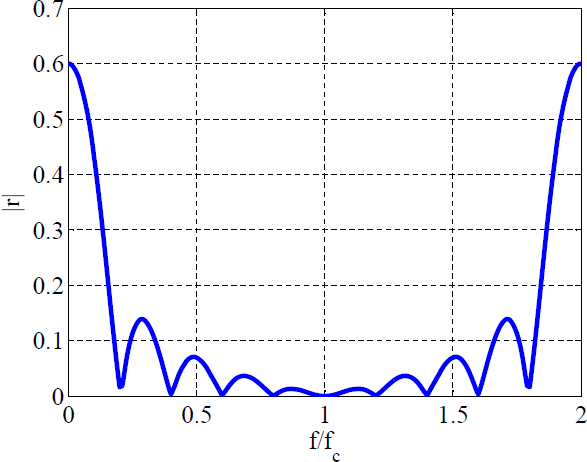
\includegraphics[width=6cm]{./bilder/rfdesign_multistage_lambda-4_transformer_result.png}
    } 
& \parbox{12cm}{
    \subsubsection{Anpassung durch Übertragungsleitungen \formelbuch{37}}

	\subsubsection{Lambda/4 Wandler (Transformer) \formelbuch{39}}
	Für gewünschte Frequenz wird der Betrag des Reflexions-Koeffizient auf ein
	Minimum verringert. \\
	Für eine einzelne Lambda/4 Leitung gilt $Z_{in} = \dfrac{Z_W^2}{Z_L}
	\Rightarrow Z_W = \sqrt{Z_{in} \cdot Z_L}$  \\
	
    Impedanz: $Z_k = \left(\frac{R_L}{R_S}\right)^{\frac{k-n-1}n} R_L$  bzw. \\
    Wellenimpedanz: $Z_{wk} =
    \sqrt{Z_{k+1} Z_k} = \left(\frac{R_L}{R_S}\right)^{\frac{2k-2n-1}{2n}} R_L$ 
	} 
\end{tabular} \\
 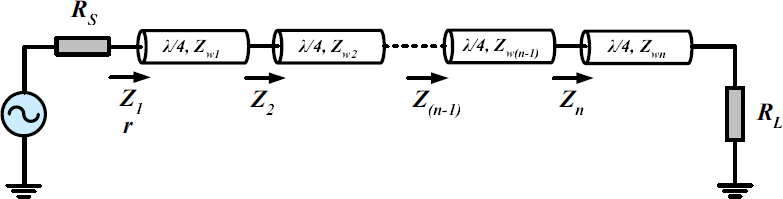
\includegraphics[height=3.6cm]{./bilder/rfdesign_multistage_lambda-4_transformer.png}
\newpage

\subsection{HF-Messungen \formelbuch{44}}
\subsubsection{Leistungssplitter, Kombinierer (Power splitter/combiner)
\formelbuch{45}}
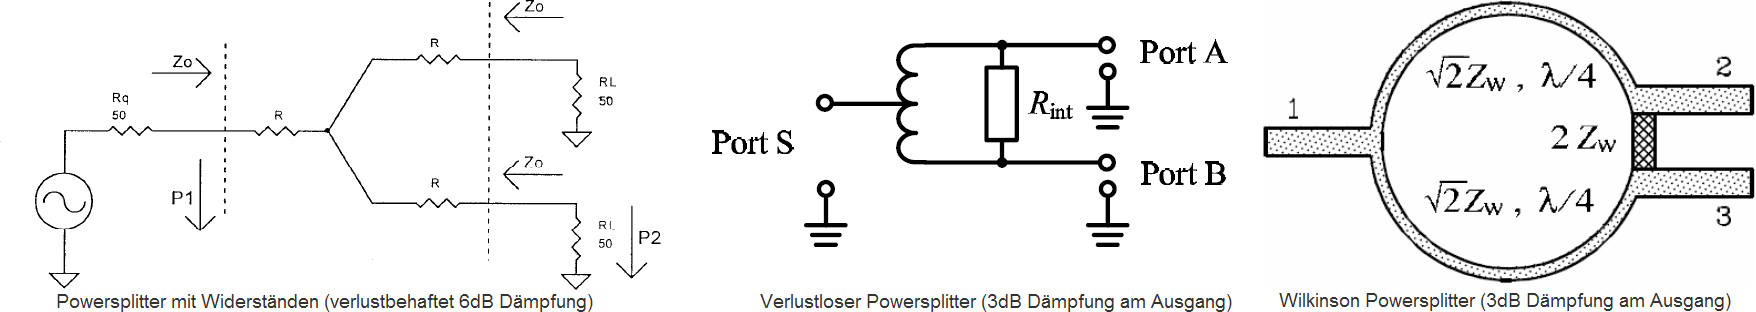
\includegraphics[width=19cm]{./bilder/rfdesign_powersplitter.png}\\
Es muss auf Impedanzanpassung geachtet werden. Die Leistungssplitter können
auch als Kombinierer gebraucht werden, dann werden die Ausgänge des Splitter zu
Eingängen und der Eingang zum Ausgang.\\
S-Matrix des Wilkinson Splitters: $S = \frac{-j}{\sqrt 2} \begin{bmatrix} 
         0 & 1 & 1 \\
         1 & 0 & 0 \\
         1 & 0 & 0          \end{bmatrix}$

\subsubsection{Richtkoppler (Directional Coupler) \formelbuch{46}}
\begin{tabular}{ll}
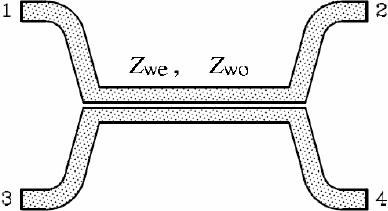
\includegraphics[width=3cm]{./bilder/rfdesign_directional_coupler.png}
  & \parbox{15cm}{
    Der Richtkoppler dient dazu, aus einer Leitung (Hohlleiter oder Koaxialkabel) einen Teil der darin laufenden elektromagnetischen Wellen richtungsabhängig abzuzweigen.
    Richtkoppler werden hierzu in die elektrische Leitung eingefügt und koppeln
	einen Teil der auf der Leitung laufenden Hochfrequenz-Leistung aus. Dabei kann
	der Anteil der vor- und rücklaufenden Welle selektiert und oft getrennt
	erfasst werden. \\
	$k = \frac{Z_{we} - Z_{wo}}{Z_{we} + Z_{wo}}$ \qquad $\kappa = \sqrt{1-k^2}$
	\qquad $S = \begin{bmatrix} 
         0        & -j\kappa & k        & 0        \\
         -j\kappa & 0        & 0        & k        \\
         k        & 0        & 0        & -j\kappa \\
         0        & k        & -j\kappa & 0        \\
         \end{bmatrix}$ \\
    $k$: Kopplungsfaktor; $Z_{we}$ bzw. $Z_{wo}$: Impedanz gegenüber
    Gleichtakt- bzw. differenziellen Signalen \\
    
    \begin{tabular}{|ll|ll|ll|}
    \hline
    return loss & $RL = -20\log |s_{11}|$
        & through loss & $T = -20\log |s_{21}|$
        & coupling & $C = -20\log |s_{31}|$ \\
    \hline
    isolation & $I = -20\log |s_{41}|$
        & directivity & $D = I-C$
        & &\\
    \hline
    \end{tabular}
    }
\end{tabular}


\begin{tabular}{lll}
\textbf{Branch-line coupler \formelbuch{47}}
    & \textbf{Rat-race divider \formelbuch{47}}
    & \textbf{Circulator \formelbuch{48}} \\
\parbox{5.5cm}{
    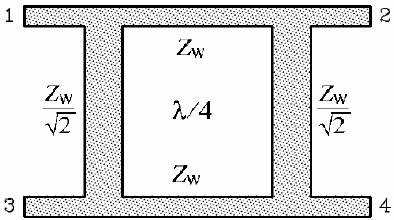
\includegraphics[width=5cm]{./bilder/rfdesign_branch_line_divider.png}\\
    Für Auskopplung von 3dB.\\
    $S = \frac{-1}{\sqrt 2} \begin{bmatrix} 
         0 & 0 & j & 1 \\
         0 & 0 & 1 & j \\
         j & 1 & 0 & 0 \\
         1 & j & 0 & 0 \\
                            \end{bmatrix}$\\
    }
& \parbox{5.5cm}{
    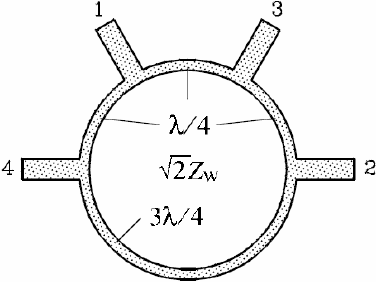
\includegraphics[width=5cm]{./bilder/rfdesign_rat-race_divider.png}\\
    $S = \frac{-j}{\sqrt 2} \begin{bmatrix} 
         0 & 0 & 1 & 1 \\
         0 & 0 & 1 &-1 \\
         1 & 1 & 0 & 0 \\
         1 &-1 & 0 & 0 \\
                            \end{bmatrix}$
    }
& \parbox{5.5cm}{
    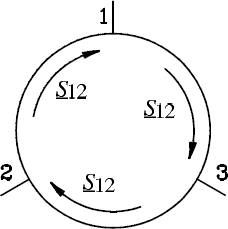
\includegraphics[width=4cm]{./bilder/rfdesign_circulator.png}\\
    Leistung wird vom einen zum nächsten Port transferriert, aber nicht zurück
    }
\end{tabular}

\newpage
\section{Kanalzugriff und Modulation \formelbuch{51}}
\subsection{Kanalzugriff}
	Den Kanalzugriff muss nur für Systeme mit mehreren unterschidlichen Sender bzw.
	Empfängern geregelt werden. Folgende Möglichkeiten bestehen:\\

\subsubsection{FDMA - Frequency Division Multiple Access - Frequenz-Multiplexing
\formelbuch{52}} Prinzip:\\Jeder Benutzer sendet auf einer zugewiesenen Frequenz mit einer
		definierten Bandbreite.\\
		Einsatzort:\\FM, aber auch GSM im Up-, wie auch im Downlink-Band (siehe
		Bild)\\
\subsubsection{TDMA - Time Division Multiple Access - Zeit-Multiplexing
\formelbuch{52}}

\begin{tabular}{ll}
\parbox{11cm}{
		Prinzip:\\Jeder Benutzer bekommt einen bestimmten Zeitschlitz, um in
		diesem Pakete senden zu können. Nach einer gewissen Zeit (Frame) wiederholt sich das
		ganze\\
		Einsatzort:\\zB. GSM: In einem Frame von 4.615ms hat es jeweils 8
		Teilnehmern (siehe Bild).}
    & \parbox{9cm}{
        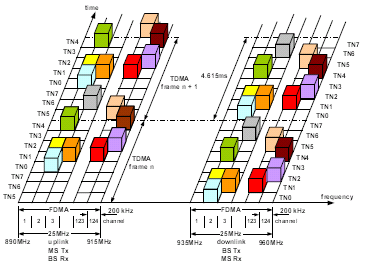
\includegraphics[width=6cm]{./bilder/modulation_TDMA.png}
        } \\
\parbox{11cm}{
		Speziell: ALOHA\\
		Für die Zuordnung der Zeitschlitze für einen neuen Teilnehmer meldet sich
		dieser zuerst bei der Basisstation. Dabei kann es zu Kollisionen mit anderen
		Teilnehmern kommen. Erneutes Melden bei der Basisstation erfolgt beim
		ALOHA-Prinzip erfolgt nach einer zufällige Zeitdauer, womit die erneute
		Kollision vermieden wird.} 
	& \parbox{9cm}{
	    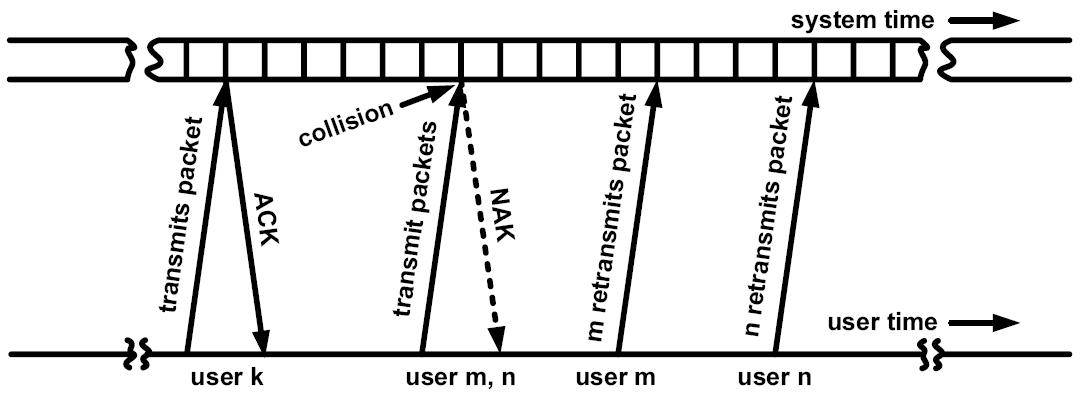
\includegraphics[width=6cm]{./bilder/modulation_aloha.png}
	    }
\end{tabular}

\subsubsection{CDMA - Code Division Multiple Access - Code Multiplexing
\formelbuch{53}} 
Prinzip:\\
Die Trägerfrequenzen werden mit Hilfe eines Codes zeitlich variiert. Durch eine
Korrelation mit demselben Codes kann man die richtigen Daten auch bei
Überlagerungen wieder herausfiltern. Deshalb können viele Sender bzw. Empfänger
auf demselben Frequenzband arbeiten. CDMA brauch jedoch durch das
Frequenzhopping auch mehr Bandbreite.\\
Vorteil/Nachteile:\\
+ Die Daten sind nur für die Empfänger mit den richtigen Codes sichtbar.\\
+ Sicher gegen Frequenzlöcher (da CDMA eine grosse Bandbreite benutzt).\\
+ Störsicher gegen schmalbandige Störsignale. \\
+ Bei wenigen Teilnehmern sehr gute SNR\\
+ Gut für unkoordinierte Teilnehmer (da keine Absprachen bezüglich
Zeitschlitz, Kanalfrequenz, etc. nötig sind)\\
- Schlechtes Near-Far-Verhalten
(wenn ein starker (naher) Teilnehmer einen schwachen (fernen) unterdrückt). \\
	

\subsubsection{OFDM - Orthogonal Frequency Division Multiplexing
\formelbuch{55}}

\begin{tabular}{ll}
\parbox{12cm}{
Funktioniert ähnlich wie FDMA, nur werden hier zueinander orthogonal stehende
Trägersignale verwendet, wobei jeder Träger ein Symbol (ein oder mehrere Bits)
repräsentiert. Laut Definition ist dann: \\
$  \int_0^{T_S} \sin (2\pi f_i t)\sin (2\pi f_j t) dt = 
  \left\{\begin{array}{l@{\,\,\,\,} l}
         0 , &   i\not = j, \\ 
         1 , &   i = j .   \end{array} \right.$\\
Daraus folgt, dass die bei FDMA übliche Sicherheitsabstände zwischen den Trägern
null sind. 
       } 
&
\parbox{6cm}{
    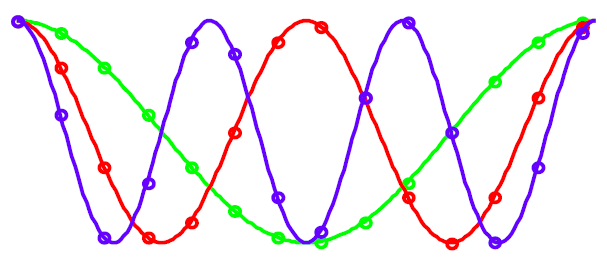
\includegraphics[width=6cm]{./bilder/modulation_OFDM-orthogonal.png}\\
    \small Orthogonalität der Träger
}       
\end{tabular}
\begin{center}
    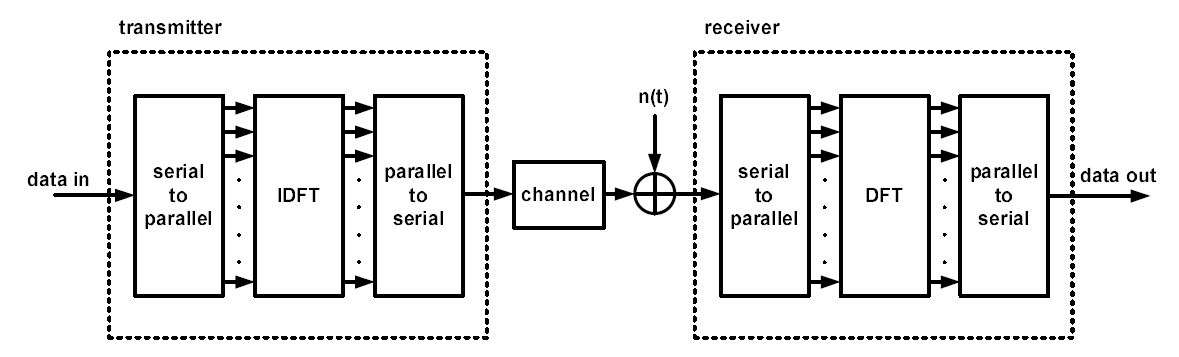
\includegraphics[width=15cm]{./bilder/modulation_OFDM-schematic.png}\\
    \small Blockschaltbild - OFDM Sender und Empfänger
\end{center}

\begin{tabular}{lll}
\parbox{4cm}{
$$\frac W{B_{\text{coh}}} \ll N_c \ll WT_{\text{coh}} $$ 
$$ T_{\text{coh}} < \dfrac{N_c}{R} = T_{\text{Subcarrier}} $$
       } 
&
\parbox{5cm}{
   $W$: Gesamtbandbreite \\
   $\dfrac{W}{N_C}$: Subcarrier Bandbreite \\
   $R$: Symbolrate (gesamtes Band)
}       
&
\parbox{9cm}{
   $N_C$: Anzahl Subcarrier bzw. Kanäle \\
   $B_{\text{coh}}$: Kohärenzbandbreite \\
   $T_{\text{coh}}$: Kohärenzzeit (Zeitinvarianz Übertragungskanal)
}       
\end{tabular}

Im Vergleich zur seriellen Übertragung ergibt sich bei der gleichen
Übertragungsrat eine viel längere
Symbolzeit, da die Daten parallel übertragen werden ergibt. Dies
ermöglicht es gegenüber Einträgerverfahren, viel weniger Bandbreite zu nutzen.
\\

Problem der \textbf{Multidimensional Interference (MDI)}:
\begin{liste}
    \item \textbf{Intersymbolic Interference (ISI)} \\
            Symbole überlappen sich im Zeitbereich (wegen Faltung mit Impulsantwort des Kanals - Laufzeit, Echo, usw.)
    \item \textbf{Inter Channel Interference (ICI)} \\
            Subcarrier sind nicht mehr orthogonal. \\
\end{liste}

\begin{tabular}{lll}
	\parbox{6cm}{ 
    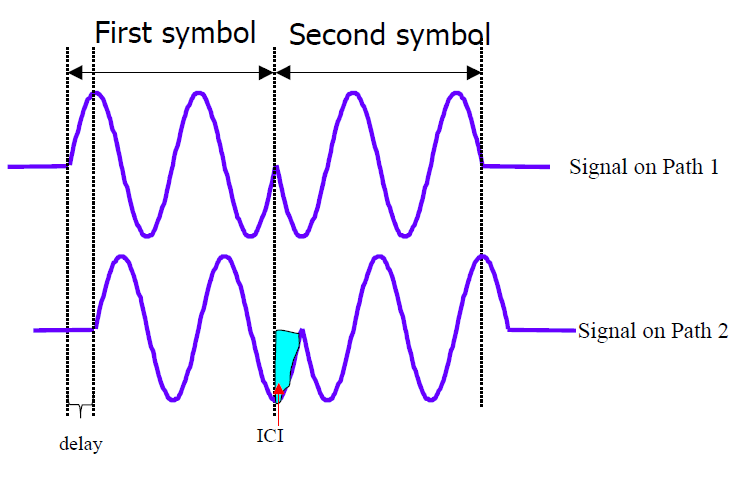
\includegraphics[width=6cm]{./bilder/modulation_OFDM-ICI.png}\\
	}    
	& \parbox{6cm}{Ein nicht-sinusförmiges Signal (Bild links) hätte mehrere/höhere
	Frequenzkomponenten zur Folge, welche in andere Subcarrier überlappen würden -
	\textbf{ICI}. Um dies zu verhindern wird das Signal mit einem sogenannten \textbf{Cyclic
	Prefix} (Bild rechts) versehen, sodass ein reines sinusförmiges Signal
	resultiert. \\	
	} &
	\parbox{6cm}{
	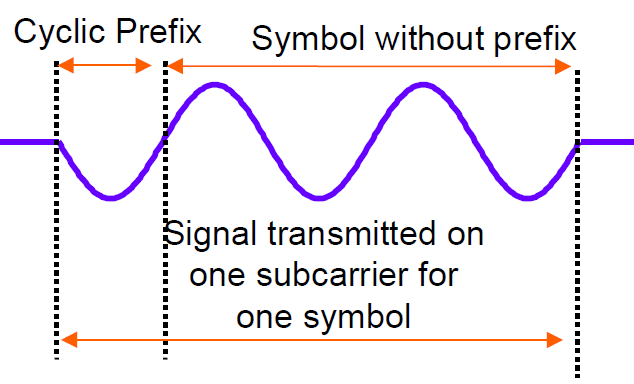
\includegraphics[width=6cm]{./bilder/modulation_OFDM-prefix.png}\\ }       
\end{tabular}


\subsection{Modulation}
Die analogen continuierlichen Modulationsarten wie AM, FM und PM werden hier
nicht behandelt. Es wird von digitalen Daten ausgegangen.

\subsubsection{Komplexes Basisband \formelbuch{57}}
Generell ist ein RF- Signal symmetrisch bezüglich des Nullpunktes
($A_1=A_{-1}$)nicht jedoch bezüglich des RF Trägers. Dies hat zur Folge, dass
das demodulierte Signal nicht mehr symetrisch zu Null ist, was bedeutet, dass
es ein komplexes Spektrum ist. $s_{RF}(t)=\Re(s_{bb}(t)e^{j2\pi f_{RF}t})$\\
\begin{tabular}{lll}
	\parbox{5cm}{
		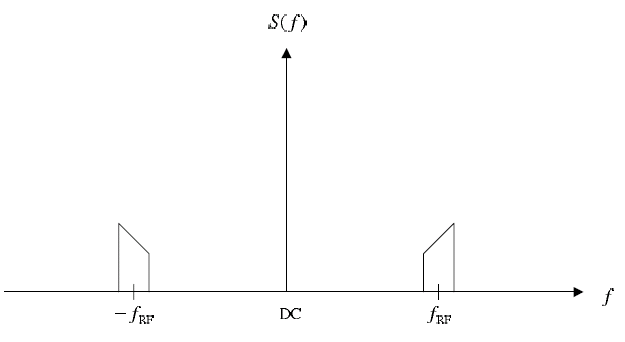
\includegraphics[width=5cm]{./bilder/modulation_RFSpektrum.png}
	}
	&$\Longrightarrow$
	&\parbox{5cm}{
		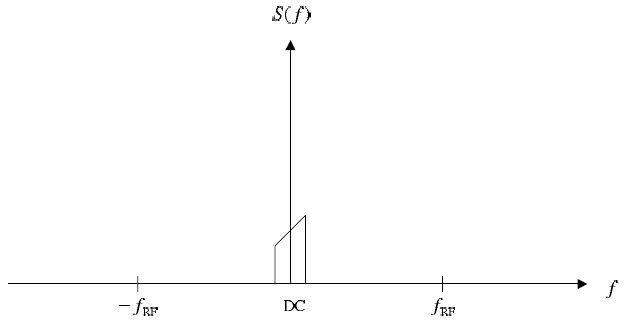
\includegraphics[width=5cm]{./bilder/modulation_BBSpektrum.png}
	}
\end{tabular}

\subsubsection{BPSK - Binary Phase Shift Keying  \formelbuch{58}}
\begin{tabular}{ll}
	\parbox{10cm}{
		\begin{tabular}{ll}
			BPSK&= 2-PAM \\
			Phase $\in \{-180^o, 0$\} &= Amplitude $\in \{-1, 1\}$
		\end{tabular}\\
		Bild rechts zeigt Amplitude und Phase des Basisbandes genau zur sampling
		time.\\
	}
	&
	\parbox{5cm}{
		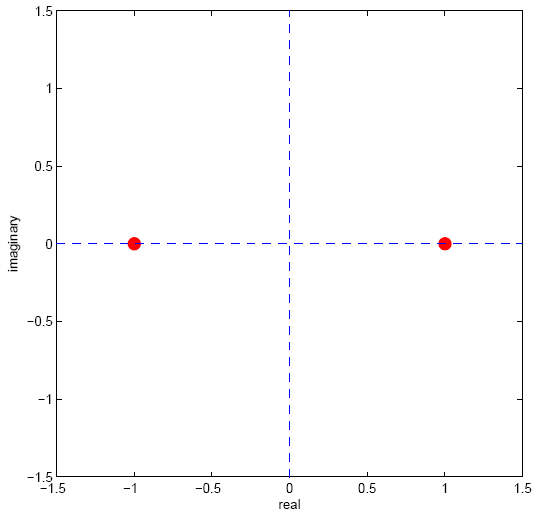
\includegraphics[width=5cm]{./bilder/modulation_constellationBPSK.png}
	}
\end{tabular}
\subsubsection{M-PAM - Pulse Amplitude Modulation \formelbuch{59}}
M kommt von M- Zuständen, welche die Amplitude annehmen kann. Dadurch können
$N=\log_2(M) [\frac{bits}{Symbol}]$ übertragen werden. Durch die Abstufung wird
die Effizienz gesteigert. Da PAM ein reelles Spektrum besitzt ist auch das
RF-Signal symmetrisch zum Träger, was jedoch die Bandbreiteneffizient stark
vermindert. Mögliche Verbesserungen:\\
\begin{liste}
	\item Zusätzlicher Imaginäranteil $\Longrightarrow$ QAM
	\item Grösseres M (Nachteil: grössere Fehlerwahrscheindlichkeit und immernoch
	symetrisch)
	\item Eliminierung des einen Frequenzbandes(z.B mit SSB)
\end{liste}

\subsubsection{M-QAM - Quadratur Amplitude Modluation \formelbuch{61}}
\begin{tabular}{ll}
\parbox{10cm}{
	Bei QAM wird die Phase und Amplidue verändert. Um eine optimale Ausnützung zu
	erhalten soll $M=2^n$ gewählt werden, wobei $n \epsilon \mathbb{N}$ und 
	$n=N=\frac{bit}{Symbol}$ist.\\
	Falls n gerade dann ergibt es ein vollständiges Viereck.\\
	Bei n ungerade ergibt sich ein Viereck ohne die Ecken.\\
	Spezialfall: 4- QAM = QPSK\\
	Das Problem für die MobKom an QAM ist, dass sich die Amplitudedämpfung sehr
	stark und relativ schnell ändern kann. Deshalb kann man keine Information als
	Amplitudenänderung senden, was dann nur noch eine Phasenverschiebung (M-PSK)
	zur Folge hat.} 
	& \parbox{8cm}{
	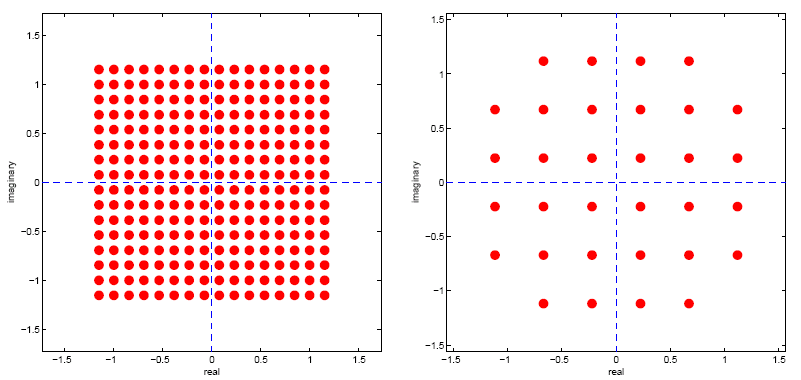
\includegraphics[width=8cm]{./bilder/modulation_constellationQAM.png}\\ 256-QAM und 32-QAM
}
\end{tabular}

\subsubsection{M-PSK - Phase Shift Keying \formelbuch{63}}
\begin{tabular}{ll}
\parbox{10cm}{
Spezielle Formen:\\
\begin{liste}
 \item Bei \textit{D}PSK kommt es nicht mehr auf die
	absolute Phase an, sondern nur noch auf den Phasensprung von Symbol zu Symbol
	(z.B. je $\frac{\pi}{4}$). So ist keine Referenz zur Nullphase nötig.
 \item \textit{$\frac{3\pi}{8}$} oder \textit{EDGE-Modulationschema} wird bei
 GSM eingesetzt. Der Vorsatz \textit{$\frac{3\pi}{8}$} bedeutet, dass zu
 einem normalen Phasensprung (hier $n \frac{\pi}{4}$ nochmals einen Offset
 von $\frac{\pi}{8}$ hinzu kommt. Dies hat zur Folge, dass die komplexe
 Amplitude nie null wird. (siehe Bild)
\end{liste}


}
&\parbox{6cm}{
    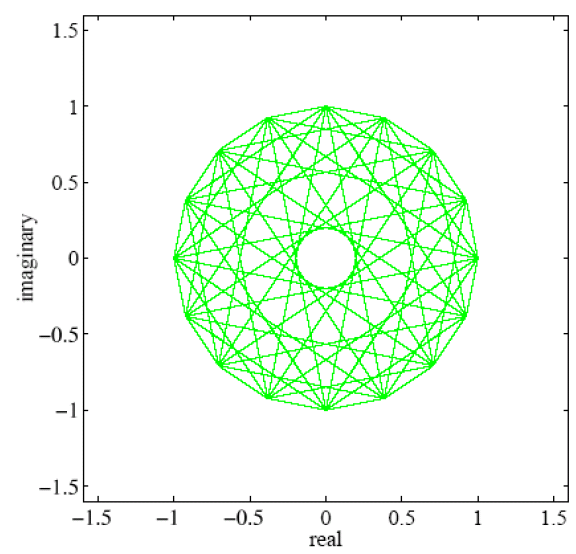
\includegraphics[width=6cm]{./bilder/modulation_constellationEDGE.png}\\
    $\frac{3 \pi}{8}$ 8-PSK

}
\end{tabular}

\subsubsection{Gray- Code \formelbuch{65}}
\begin{tabular}{ll}
	\parbox{8cm}{
		Der Vorteil des Gray Codes gegenüber der normalen binären Codierung ist, dass
		bei einem Fehler nur ein Bit falsch wird und nicht gerade alle, wie das Bild
		rechts zeigt.\\
        Bsp. aus Prüfung (12. März 2007): Vergrösserung des BER, wenn bei QPSK
        die binäre Standardcodierung statt der Gray-Codierung verwendet wird.
        
        Gray: BER = SER/2 \\
        Binär: BER = SER/2 + SER/4 \\
        Verschlechterung: $\Rightarrow 3/2$   \\ \\
        
        Für Gray-Code gilt: $\text{BER} \approx
        \dfrac{\text{SER}}{n_{\text{bits}}}$ } &\parbox{10cm}{
		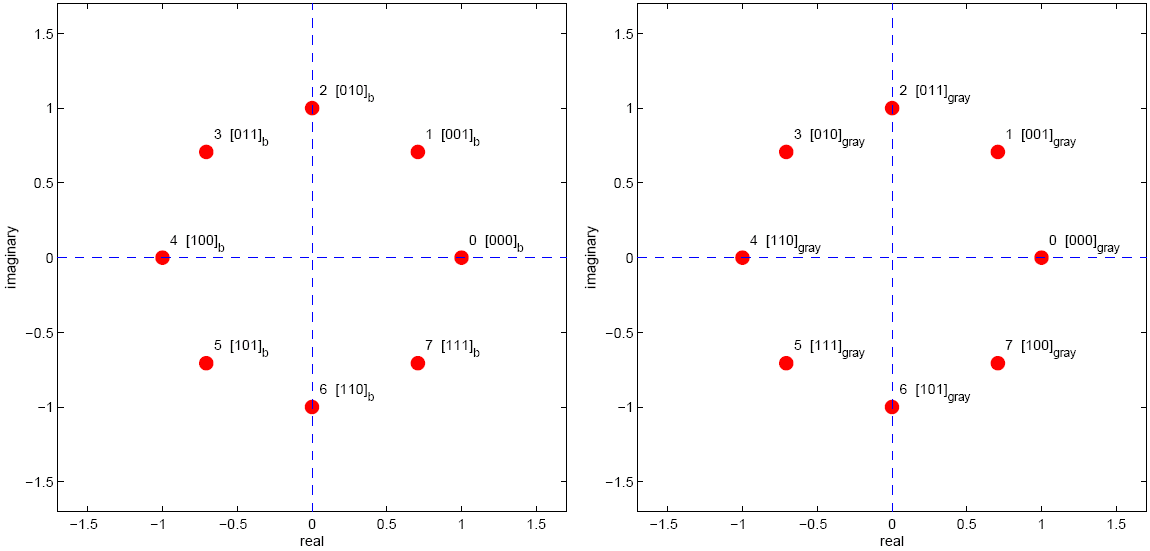
\includegraphics[width=10cm]{./bilder/modulation_PSKmitGray.png}\\
		8-PSK ohne bzw. mit Gray- Code
	}
\end{tabular}

\begin{tabular}{ll}
	\parbox{9cm}{
		\subsubsection{FSK - Frequency Shift Keying \formelbuch{65}}
		Bei FSK wird ein binäres Signal frequenz-moduliert. Das heisst,
		es switscht (hihi) zwischen zwei Frequenzen, dies wird meist mit Hilfe eines
		VCO gemacht.\\
		Kenngrösse ist der Modulations Index: \\
		$h=\dfrac{\Delta f}{f_{\text{data}}}=\dfrac{f_{\text{max}} -
		f_{\text{min}}}{f_{\text{data}}} =\dfrac{n_{\text{T-max}} -
		n_{\text{T-min}}}{n_\text{T}}$ \\ Bei einem \textbf{h von 0.5 }spricht man von
		\textbf{Minimum Shift Keying (MSK)} oder \textbf{Fast} Frequency Shift Keying
		\textbf{(FFSK)}. Trägerfrequenzen können orthogonal sein, solange der
		Modulationsindex das Minimum $h_{\text{min}}$ nicht unterschreitet. \\ $h_{\text{min}} =
		\begin{cases} 1   & \text{unkohärente Detektion} \\                                
                                0.5   & \text{kohärente - phase
                                synchron - Detektion} \end{cases}$\\
        Für unkohärente Detektion sind die beiden Träger orthogonal, wenn gilt:
        \\
        $    \Delta f = \frac{1}{T_{\text{data}}} \cdot n , \qquad n \in \lbrace
        1, 2, 3, \ldots \rbrace $
	}
	&\parbox{9cm}{
	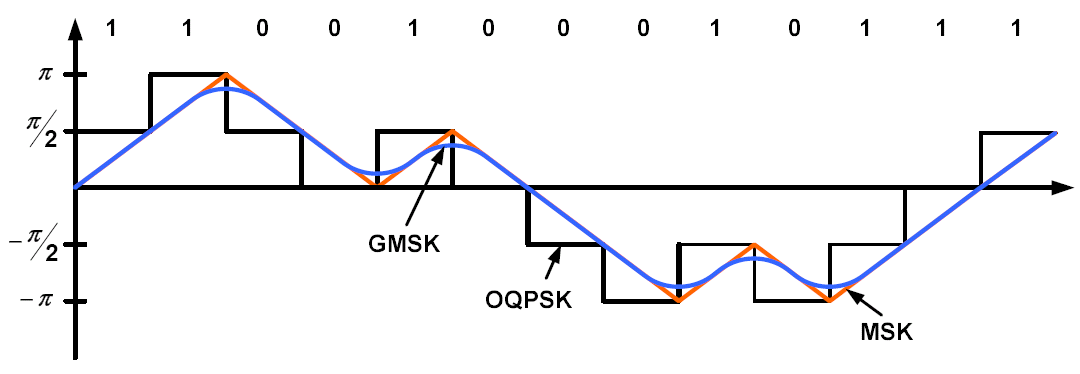
\includegraphics[width=9cm]{./bilder/modulation_phasenverschiebungGMSK_MSK.png}\\
	Phasenverschiebung des MSK bzw GMSK. }
\end{tabular}
     
        
\subsubsection{GMSK - Gaussian Minimum Shift Keying \formelbuch{67}}
Das GMSK ist ein MSK mit einem gauss'schen premodularen Filter. Es besitzt eine
konstante Amplitude und eine grosse spektrale Effizient.
        

\subsubsection{OQPSK - Offset Quadratur Phase Shift Keying \formelbuch{75, 68}}
Das OQPSK ist eine Sonderform der Quadraturphasenmodulation
	
	
\subsection{Modulationskriterien}
Es gibt 3 Wege um die Fehlerwahrscheinlichkeit
herauszufinden:
\begin{liste}
	\item Austesten und messen (dauert bei kleiner Fehlerwahrscheinlichkeit so
	lange, bis ein vernünftiges Resultat erreicht wird).
	\item Simulieren (dazu ist ein gutes Model nötig, kann unter Umständen gleich
	lange dauern wie austesten).
	\item Analystisch mit Symbol- und Biterrorrate.
\end{liste}
\subsubsection{SER - Symbolfehlerrate \formelbuch{70}}
\begin{tabular}{ll}
\parbox{8cm}{
    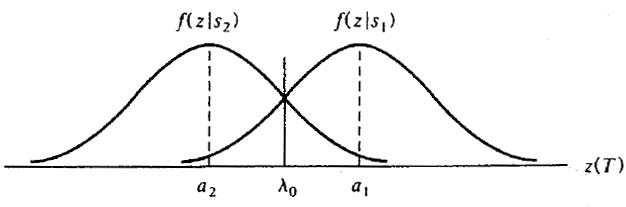
\includegraphics[width=8cm]{./bilder/modulation_AWGN.jpg}
    }
& \parbox{9cm}{
	Die Symbolfehlerrate wird unter anderem verursacht durch das thermische
	Rauschen (AWGN). Dieses hat die Energie\\ 
	$\sigma^2=\frac{N_0}{2}$ \\
	\\
	Die Fehlerwahrscheinlichkeit ist $P_E=Q(\sqrt{\frac{2 E_S}{N_0}})$ mit $a_1 =
	E_S, a_2 = -E_S$ und $\lambda_0 = 0$\\
    }
\end{tabular}

\small
\renewcommand{\arraystretch}{0.6}
% \hspace*{10mm}
\begin{tabular}[ht]{|l|l|l|l|l|}\hline
Modulation & levels/ & normalized & SER (AWGN)
           & Comments \\
scheme     & range   & amplitude  &     &          \\
\hline \hline
%&&&&\\[-3mm]
BPSK & $\pm A$& $A=1$ &
  $Q{(\sqrt{\frac{2E_s}{N_0}})}$ & \\[2mm]  \hline
%&&&&\\[-3mm]
DPSK & $\pm A$& $A=1$ &
  $2Q(\sqrt{\frac{2E_s}{N_0}})$ & coherent \\ 
  &&& $\frac{1}{2}e^{-\frac{E_s}{N_0}}$ & noncoherent\\[2mm] 
\hline
%&&&&\\[-3mm]
QPSK & $(\pm 1\pm j)A$ & $A=\frac{1}{\sqrt{2}}$&
  $ 1-\left(1-Q(\sqrt{\frac{E_s}{N_0}})\right)^2$ & coherent \\[2mm] \hline
%&&&&\\[-3mm]
DQPSK &$(\pm 1\pm j)A$ & $A=\frac{1}{\sqrt{2}}$& 
  $ 2\left(1-\left(1-Q(\sqrt{\frac{E_s}{N_0}})\right)^2\right)$ & coherent \\
&&&  $\frac{1}{2}e^{-\frac{E_s}{2N_0}}$ & noncoherent\\[2mm] \hline
%&&&&\\[-3mm]
$M$-PSK & $ \frac{1}{M}\sum_{m=1}^{M}
             A\delta\left(x- e^{j(2m-1)\frac{\pi}{M}}\right),$ & $A=1$&
  $ \leq 2Q(\sqrt{\frac{2E_s}{N_0})\sin\frac{\pi}{M}})$
  & coherent \\
& $\qquad \qquad \qquad \qquad \,\,\,\,\, m\le M$ &&& \\[2mm] \hline
%&&&&\\[-3mm]
$M$-PAM & $\pm (2m-1)A,\quad m\le M/2$ & $A=\sqrt{\frac{3}{M^2-1}}$ &
  $2\frac{M-1}{M}Q\left(\sqrt{\frac{E_s}{N_0}}\sqrt{\frac{6}{M^2-1}}\right)$ &
  \\[2mm]  \hline
%&&&&\\[-3mm]
$M$-QAM & $(\pm (2m-1)\pm j(2n-1))A,$ & $A=\sqrt{\frac{3}{2(M-1)}}$ 
  &$1-\left(1-2\frac{\sqrt{M}-1}{\sqrt{M}}Q\left(\sqrt{\frac{E_s}{N_0}}
   \sqrt{\frac{3}{M-1}}\right)\right)^2$ & \\
& $\qquad \qquad \quad m,n\le \sqrt{M}/2$ &&& \\[2mm] \hline
%&&&&\\[-3mm]
2-FSK &$\Delta f=h\cdot \frac{1}{T},\, h_{\min}=0.5$ &&
  $Q(\sqrt{\frac{E_s}{N_0}})$ 
  & orthogonal, coherent  \\
& \qquad \qquad \quad $h_{\min}=1$ &&
  $\frac{1}{2}e^{-\frac{E_s}{2N_0}}$ 
  & orthogonal, noncoherent \\[2mm] \hline
\end{tabular}
\renewcommand{\arraystretch}{1}


\subsubsection{BER - Bitfehlerrate \formelbuch{72}}
\begin{tabular}{ll}
	\parbox{10.5cm}{
	Sobald eine Informationsrate R kleiner als die Kanalkapazität C ist, sind
	fehlerfreie Übertragungen möglich.\\
	$C= W \log_2 ( 1+\frac{S}{N}) > R$\\
	Wobei W die Bandbreite des Kanals, N die Rauschenergie $N=N_0 W$ und S die
	Signalenergie ist.
	Die Grenze ist bei $C=R \Longrightarrow E_b C$ $E_b$ ist die Bitenergie\\

	$\Longrightarrow \frac{C}{W}= \log_2(1+\frac{E_b C}{N_0 W})$\\ 

	
	\subsubsection{Spektrale Effizient \formelbuch{75}}
	Heisst wieviel Bandbreite pro Datenrate gebraucht wird.
	Die Effizient beinhaltet zwei Kriterien:
	\begin{enumerate}
	\item Wieviele Bits können in einer gegeben Bandbreite übertragen werden. Wenn
	man die Begrenzung durch die SNR beliebig erweitern indem man die Bits/Symbol
	erhöht.
	\item Wieviel das Spektrum die Nachbarn überlagert. Je nach Modulation gibts
	einen breiten Mainlobe mit schwachen Sidelobes oder umgekehrt.
    \end{enumerate}
  
    \subsubsection{Raised-Cosine-Filter \formelbuch{63}}
    $h(t) = \frac{\sin\left((t/T)\pi\right)}{(t/T)\pi}\cdot
        \frac{\cos\left(\rho(t/T)\pi\right)}{1-4\rho^2(t/T)^2}$\\
   
    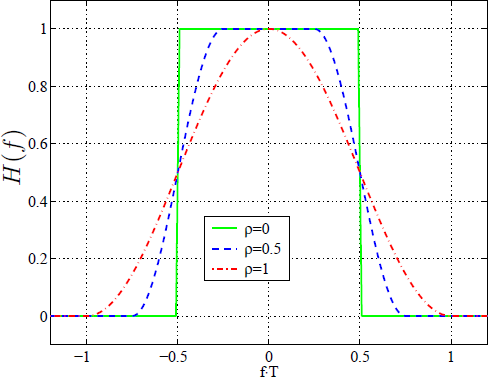
\includegraphics[width=5cm]{./bilder/modulation_raised_cosine_frequency.png}
    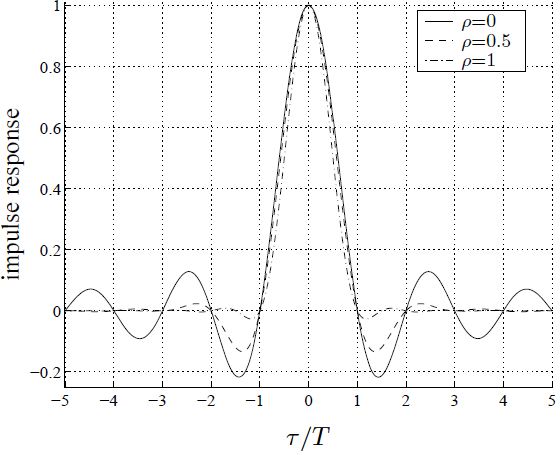
\includegraphics[width=5cm]{./bilder/modulation_raised_cosine_time.png} 
    
    Das \textbf{Root-Raised-Cosine-Filter} entspricht der Wurzel des
    Raised-Cosine-Filters und wird angewendet, wenn die Charakteristik 
    des Raised-Cosine-Filters auf Sender und Empfänger
    gleichmässig verteilt werden soll.
    } &\parbox{7cm}{
	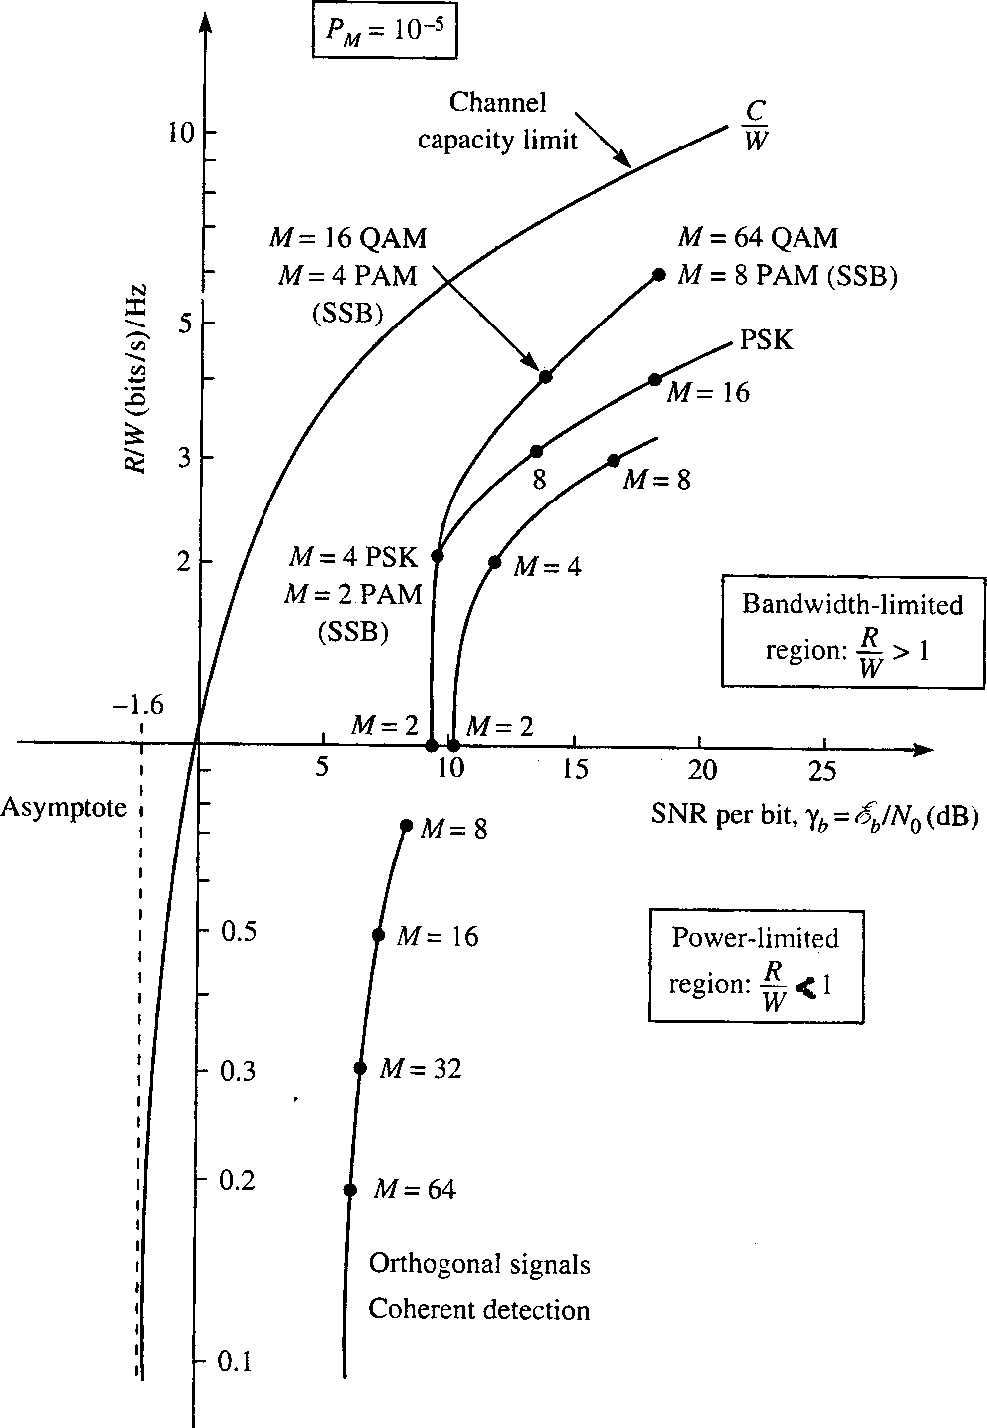
\includegraphics[width=7cm]{./bilder/modulation_SER.png}\\
	Übersicht einzelner Modulationen mit einer SER von $10^{-5}$
	}
\end{tabular}

\newpage



\section{HF-Komponenten \formelbuch{77}}
\subsection{Verstärker \formelbuch{77}}
Bei Verstärkern unterscheidet man zwischen \textbf{Low-Noise Amplifier (LNA)} und \textbf{Power
Amplifiers (PA)}. \\
\begin{liste}
\item \textbf{LNA} - Nahe bei Empfangsantenne, tiefe Leistungen, tiefe Noise Figure (NF)
\item \textbf{PA} - Vor Sendeantenne, hohe Leistungen / Effizienz und Linearität
\end{liste}

\subsubsection{Stabilität \formelbuch{77}}
Es wird zwischen bedingter (conditional stability) und unbedingter Stabilität (unconditional
stability) unterschieden:
\begin{liste}
\item \textbf{Bedingte Stabilität} - Verstärker neigt bei gewisser Last- oder Quellimpedanz zum
Schwingen
\item \textbf{Unbedingte Stabilität} - Verstärker ist in jedem Fall stabil
\end{liste}
\vspace{.2cm}

\begin{tabular}{lll}
\parbox{9cm}{
    \textbf{Variante 1} \\
    $  k=\dfrac{1-|s_{11}|^2-|s_{22}|^2+|\Delta|^2}{2|s_{12}s_{21}|} > 1 $\\
    $  |\Delta|=|s_{11}s_{22}-s_{12}s_{21}| <1 $ \\
    \textbf{Unbedingt} stabil wenn beide Bedingungen erfüllt sind. \\
    }
& \parbox{9cm}{
    \textbf{Variante 2} \\
    $  \mu =\dfrac{1-|s_{11}|^2}%
          {|s_{22}-s_{11}^*\Delta|+|s_{21}s_{12}|} > 1 $\\
  mit $\Delta =s_{11}s_{22}-s_{12}s_{21} $ \\
    \textbf{Unbedingt} stabil wenn Bedingung erfüllt ist. \\
} \\
\end{tabular}


\begin{tabular}{lll}
\parbox{9cm}{
   \textbf{Stabilitätskreise} \\    
        Für \textbf{bedingte} Stabilität werden im Smith-Chart
        \textbf{Stabilitätskreise} (für verschiedene Frequenzen)
        eingezeichnet. Diese markieren den Bereich der Last- oder
        Quellenimpedanzen wo der Verstärker instabil wird. \\
        Diese Kreise werden durch Setzen von $|\Gamma_{\text{in}}|=1$
        oder $|\Gamma_{\text{out}}|=1$ errechnet.
        \textcolor{red}{bessere erklärung!}        
        }
& \parbox{9cm}{
        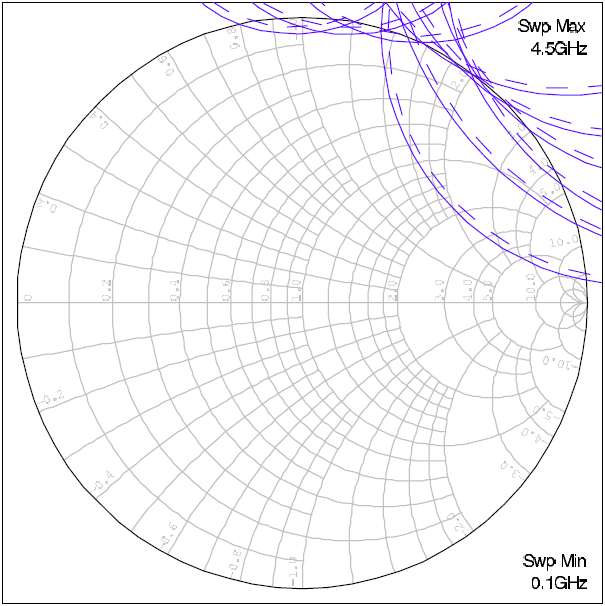
\includegraphics[height=3.5cm]{./bilder/components_amplifier_stability.png}
        }\\
\end{tabular}

\subsubsection{Verstärkung \formelbuch{79}}

\begin{tabular}{ll}
\parbox{8.5cm}{
	Im Gegensatz zum \textbf{forward gain $s_{21}$}, welcher die Verstärkung bei
	optimaler Quellen- und Lastimpedanz beschreibt, zeigt die \textbf{transducer gain $G_T$} wieviel Verstärkung,
	bedingt durch verschiedene Quelen- und Lastimpedanzen, resultiert. \\
	mit $\Gamma_S=r_s$, $\Gamma_L=r_l$ \\	
    $  G_T= |s_{21}|^2 $ bei angepasster Last- und Quellenimpedanz.\\
	} 
& \parbox{9cm}{        
        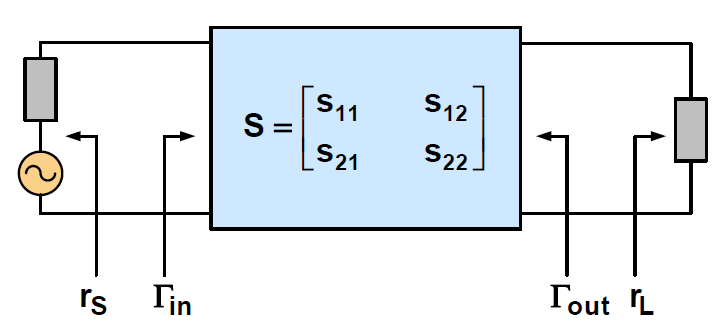
\includegraphics[height=4cm]{./bilder/components_amplifier_schematic.png}
        }\\

$  G_T= \dfrac{(1-|r_s|^2)|s_{21}|^2(1-|r_l|^2)}
   {|(1-s_{11}r_s)(1-s_{22}r_l)-s_{21}s_{12}r_sr_l|^2}; \quad $
& $  G_{T,\max}\mid_{s_{12}=0}= \dfrac{|s_{21}|^2}
   {(1-|s_{11}|^2)(1-|s_{22}|^2)} \quad$ mit $r_s=s_{11}^*$ und $r_l=s_{22}^*$\\

\textbf{Operating Power Gain}
    & \textbf{Available Power Gain} \\
$G_{op}= f(\Gamma_L)  $ 
    & $G_{av}= f(\Gamma_S) $ \\
unabhängig von Quellenimpedanz $\Gamma_S = 0$
    & unabhängig von Lastimedanz $\Gamma_L = 0$ \textcolor{red}{TODO: check this!}
\end{tabular} \\

\begin{tabular}{ll}
\parbox{9cm}{
    \textbf{Gain Circles} \\
    Für Fehlanpassungen entweder am Ein- oder Ausgang, werden im Smith-Chart Kreise für
    verschiedene Verstärkungen $g$ gezeichnet. Folgende Formeln gelten für $s_{12}=0$ \\

    $g= \dfrac{1-|r_s|^2}{|1-s_{11}r_s|^2}$ \\
    $r_s = \dfrac{g\cdot s_{11}^*}{g|s_{11}|^2+1}$ \\
    $\rho_s = \dfrac{\sqrt{g|s_{11}|^2+1-g}}{g|s_{11}|^2+1}$    \\
    
        Der Kreismitteplunkt $r_s$ liegt auf der Strecke zwischen $s_{11}^*$ und Smith-Chart
    Mittelpunkt. Der Radius beträgt $\rho_s$.  \\ 
     }
& \parbox{9cm}{        
        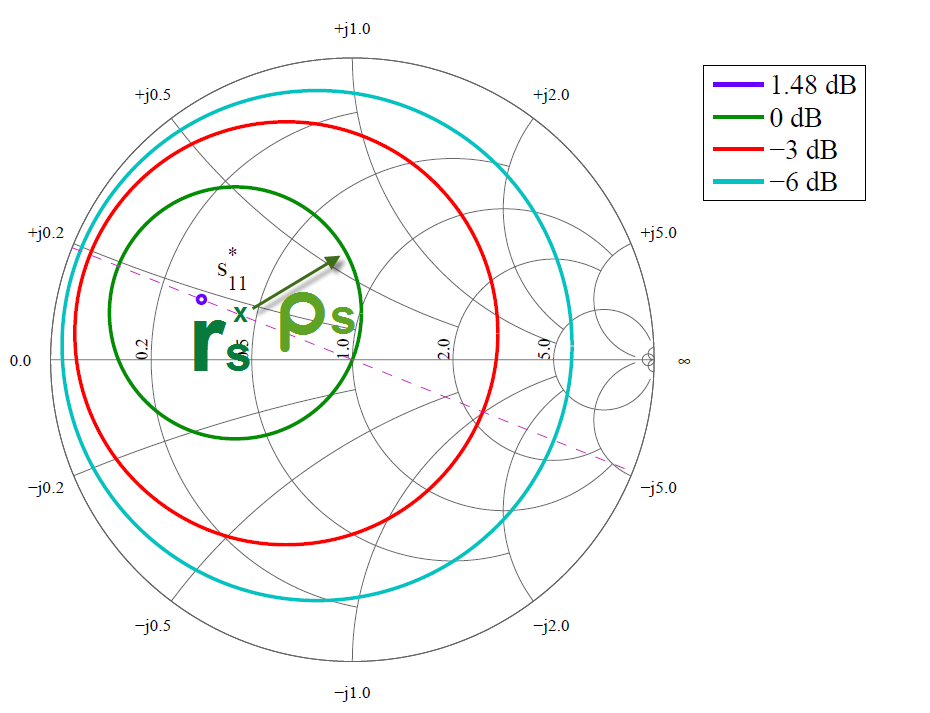
\includegraphics[width=7cm]{./bilder/components_amplifier_gain-circles.png}
        }\\
\end{tabular}


\textbf{Gründe} weshalb Verstärker die \textbf{maximale Verstärkung nicht erreicht}: \\
Fehlende Anpassung am Ein- oder Ausgang, Anpassung mit verlustbehafteten Elementen, potentielle
Instabilität.

\subsubsection{Rauschen \formelbuch{81}}
Wegen dem Eigenrauschen $\text{N}_{\text{out,total}}$ des Verstärkers ist das
$\text{SNR}$ am Ausgang des Verstärkers kleiner (also schlechter) als dasjenige am Eingang. Diese Differenz ist durch die noise figure NF (in dB)
oder den noise factor $F$ (linear) gegeben.
\vspace{0.1cm}\\
$ \boxed{F = \dfrac{\text{SNR}_{\text{in}}}{\text{SNR}_{\text{out}}} = 
\dfrac{\text{N}_{\text{out,total}}}{\text{N}_{\text{out,source}}}=
\dfrac{\text{N}_{\text{out,total}}}{\text{G}\cdot \text{N}_{\text{in}}}}
\qquad \Longleftrightarrow \qquad \boxed{\text{NF} = 10 \cdot \log_{10} (F) =
\text{SNR}_{in.dB} - \text{SNR}_{out.dB} =
\text{N}_{\text{out,total,dB}}-(\text{G}_{dB}+ \text{N}_{\text{in,dB}})}$
\vspace{0.1cm}\\
$ N_{in} = k T B \qquad \text{mit } k = 1.38 \cdot
10^{-23} \qquad (k T_0)_{dB} |_{T_0 = 290K} = -174 \text{dBm/Hz} \qquad
N_{in,dB} = (k T_0)_{dB} + 10 \log_{10} (B)$ \\
\vspace{0.1cm}
Die Bandbreite $B$ des Rauschen
$N_{in}$ ist durch das schmalbandigste Filter in einer Kaskade definiert.
\vspace{0.2cm}
Veränderung der SNR bzgl. Rauschen: $\qquad \text{SNR}_{out.dB} <
\text{SNR}_{in.dB} \qquad \text{SNR}_{out.dB} = \text{SNR}_{in.dB} - \text{NF}
= (S_{in.dB} - N_{in.dB}) - \text{NF}$

\begin{tabular}{ll}
\parbox{9cm}{
    \textbf{Kaskadierte Blöcke \formelbuch{86}} \\
    $$G = G_1 \cdot G_2 \cdot \cdot \cdot G_k \qquad G_{dB} = G_{1.dB} + G_{2.dB} + \cdot \cdot
    \cdot + G_{k.dB}$$ 
    $$F=F_1+\dfrac{F_2-1}{G_1}+ \dfrac{F_3-1}{G_1G_2}+\ldots 
       + \dfrac{F_K-1}{G_1G_2\cdots G_{K-1}}$$ 
       $$\text{Unendliche Kaskade: }F_{\infty} = F + \dfrac{F-1}{G-1} =
       \dfrac{G \cdot F-1}{G-1}$$ Für passive Komponenten gilt: $F =
       \frac{1}{G_{passive}}; G = G_{passive}$ }
& \parbox{9cm}{        
        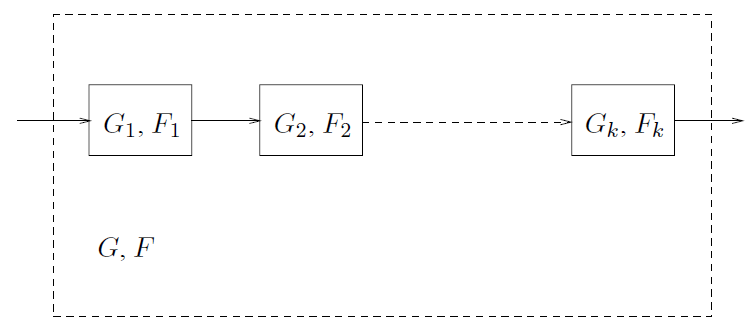
\includegraphics[width=9cm]{./bilder/components_amplifier_noise_cascade.png}
        }\\
\end{tabular}\\

Grundsätzlich \textbf{dominiert} das \textbf{erste Element} einer Kaskade die noise figure NF. Ist dessen noise factor
$F_1$ klein und die Verstärkung $G_1$ gross, so wird der gesamte noise factor $F$ klein. Dies sind
u.a. Eigenschaften von LNA-Verstärkern.\\

\begin{tabular}{ll}
\parbox{12cm}{
    \textbf{Funkelrauschen - flicker noise \formelbuch{87}} \\
    Bei tieferen Frequenzen $f$ domitiert das Funkel- oder auch 1/f-Rauschen gegenüber dem
    thermischen Rauschen. \\ \\
    \parbox{8cm}{
    \begin{tabular}{|l|l|}\hline
    Element & corner frequency $f_c$ \\ \hline \hline
    Si-bipolar transistors & 100\,Hz to 1\,kHz \\ \hline
    Si-MOSFET              & 100\,Hz to 1\,MHz \\ \hline
    GaAs-MESFET            & 1\,MHz to 50\,MHz \\ \hline
    \end{tabular}
}
    \parbox{3cm}{
    $F=F_0 \cdot \left(\frac{f_c}{f}+ 1\right)$
    }
 %\includegraphics[height=2.5cm]{./bilder/components_amplifier_noise_flicker_table.png}
     }
& \parbox{6cm}{        
        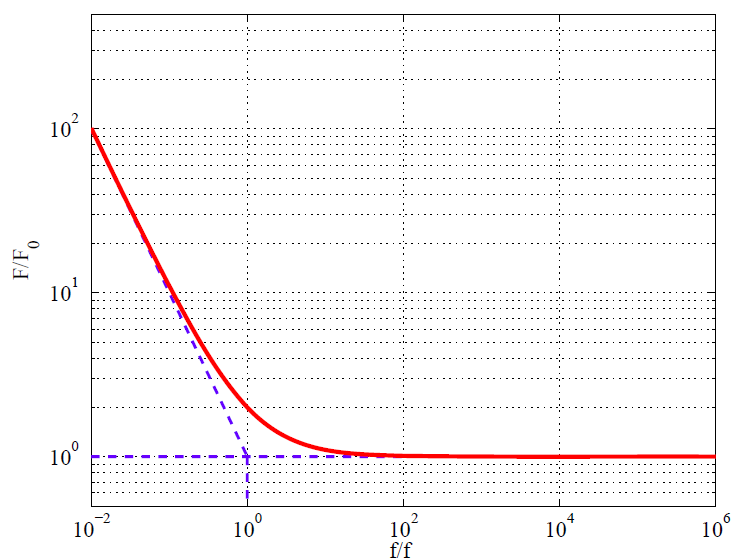
\includegraphics[height=4cm]{./bilder/components_amplifier_noise_flicker.png}
        }\\
\end{tabular}

    \textbf{Rauschmessung \formelbuch{89}}\\
    Die Rauschleistung eines Verstärkers mit Verstärkung $G$ und Bandbreite $B$
    wird bei zwei verschiedenen Temperaturen ($T_C$: Cold, $T_H$: Hot) gemessen.    
    $$ P_h = k B G(T_h+ T_E) \qquad \qquad  P_c = k B G(T_c+ T_E) \qquad \qquad 
    Y=\frac{P_h}{P_c} = \frac{T_h+ T_E}{T_c+ T_E} $$
    $$  T_E=\frac{T_h-YT_c}{Y-1} \qquad \qquad   
     F = \left(1+ \frac{T_E}{T_0}\right)
    \qquad \qquad 
    \left( \text{für } T_c = T_0 \text{ gilt}: \text{ENR} = \frac{T_h-T_0}{T_0}
     \quad \text{ und } \quad  F= \frac{\text{ENR}}{Y-1}  \right)$$
    

\subsubsection{Nichtlinearitäten \formelbuch{90}}
Reale Verstärker sind nicht perfekt und somit nicht linear. Nichtlineare Komponenten
werden Verzerrung hervorgerufen. Dies macht sich umso mehr bemerkbar, je näher
die Ausgangspegel an die Grenzen der Spannungsversorgung geraten.
$$ v_{\text{out}} = a_1 v_{\text{in}} - a_3 v_{\text{in}}^3 \quad \Longleftrightarrow \quad  
v_{\text{out}}|_{v_{\text{in}}=A \sin \omega t} = A(a_1 -\frac 34a_3A^2)\sin  \omega t
                      +\frac 14a_3A^3\sin 3\omega t$$
Die dabei entstehenden 3. Harmonischen (dreifache der Grundfrequenz) sind hierbei besonders von
Interesse. \\

\begin{tabular}{ll}
\parbox{12cm}{
    \textbf{1dB Compression Point} \\
    Beschreibt die \textbf{Eingangsleistung} bei welcher die \textbf{Ausgangsleistung}
    (durchgezogene Linie) \textbf{1dB tiefer} ist, als sie idealerweise (gestrichelte Linie) sein
    sollte. $$ A a_1 \sin(\omega t) - \frac{3 a_3 A^3 \sin(\omega t)}{4} = A a_1 \sin(\omega t) -
    1\text{dB}; \qquad \frac{A_{\text{IIP3}}}{A_{\text{1dB}}}=14.4 \text{dB}$$ }
& \parbox{6cm}{        
        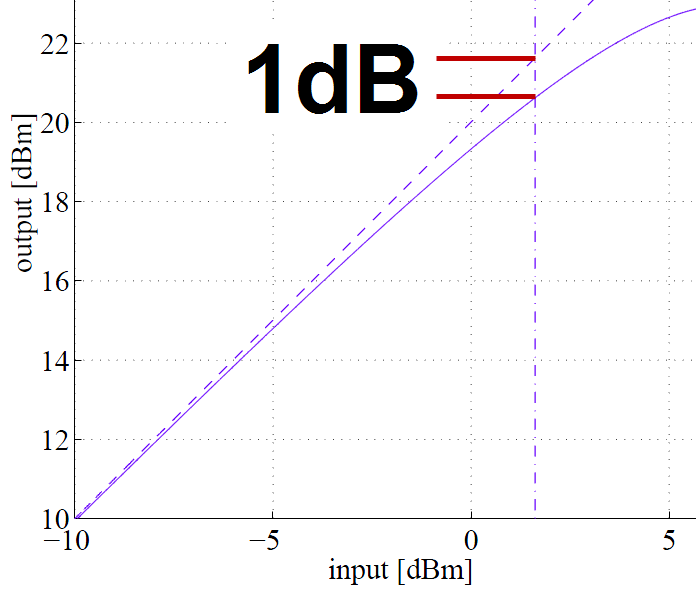
\includegraphics[height=3cm]{./bilder/components_amplifier_nonlinear_1db.png}
        }\\
\end{tabular}\\        
               
\begin{tabular}{ll}
\parbox{10cm}{
    \textbf{Third-order Interception Point OIP$_3$, IIP$_3$} \\
    Ausgangsleistung, wo die Leistung der dritten Harmoischen gleich
    derjenigen des Grundsignals (erste Harmonische) ist.
    $$ \text{HD}_3
             = P_{\text{out}}-2(\text{OIP}_3-G-(P_{\text{out}}-G))
            = 3P_{\text{out}}-2\text{OIP}_3 \quad \text{\small{(Werte in dB)}}
            $$ $$  \frac 1{\text{OIP}_{3,\text{total}}} =
  \frac 1{G_2G_3\text{OIP}_{3,1}} +
  \frac 1{G_3\text{OIP}_{3,2}} +
  \frac 1{\text{OIP}_{3,3}} \quad \text{\small{(Werte linear)}}$$
$$  \text{IIP}_{3,\text{total}} =
  \frac{\text{OIP}_{3,\text{total}}}{G_1G_2G_3} \quad \text{\small{(Werte linear)}}$$     
  Der SFDR (spurious-free dynamic range) beschreibt den Bereich des
  Eingangssignals, bei welchem keine Störungen am Ausgang auftreten -
  Signalleistung grösser Rauschleistung und Leistung dritter Harmonischen kleiner
  Signalleistung.
  $$ \text{SFDR}= \frac 23(\text{IIP}_3-N) = \frac 23(\text{IIP}_3-(-174\,\text{dBm}
                 +10\log_{10} B + \text{NF})) $$
  
     }
& \parbox{8cm}{        
        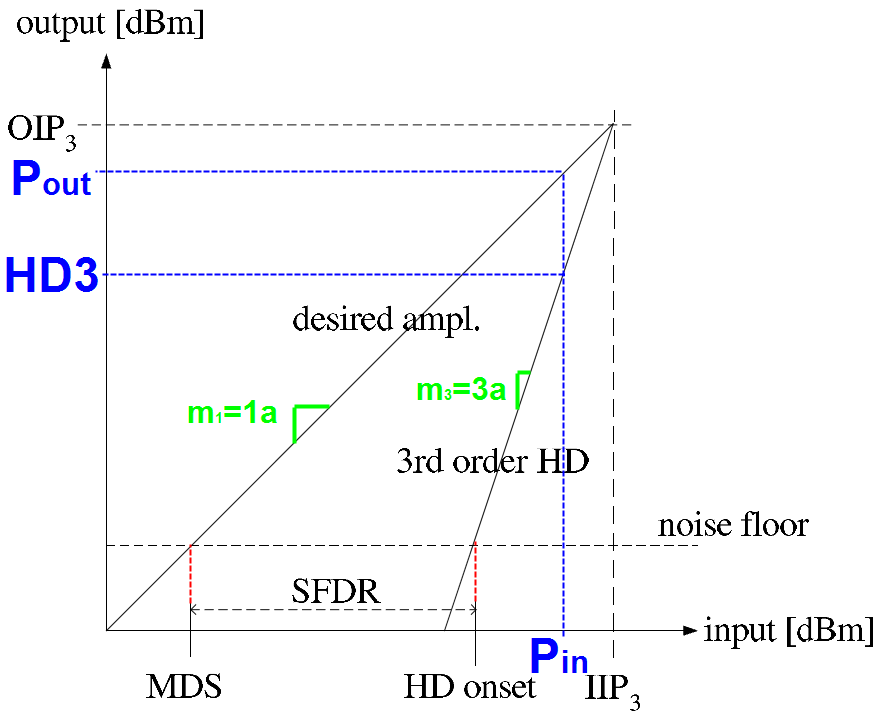
\includegraphics[width=9cm]{./bilder/components_amplifier_nonlinear_xip3.png}
        }\\
\end{tabular}\\                      

\subsection{Baluns - Symmetrieglied \formelbuch{93}}
Wandelt zwischen einem \textbf{symmetrischen (balanced)} und einem \textbf{assymetrischen (unbalanced)} Signal. \\
Symmetrische (balanced) Leitungen führen \textbf{zwei} gegenüber Ground symmetrische Signale. \\
\begin{tabular}{lll}
\parbox{9cm}{
    \textbf{Voltage Balun}\\
    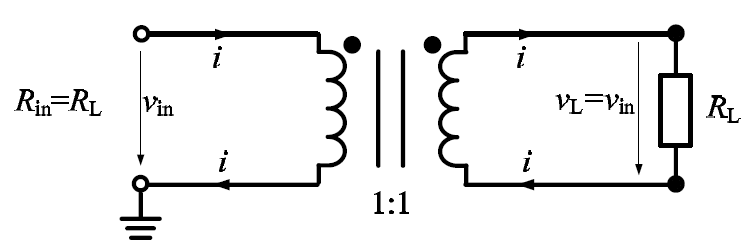
\includegraphics[width=8.5cm]{./bilder/components_voltage_balun.png}
    }
& \parbox{9cm}{
    \textbf{Current Balun} \\
    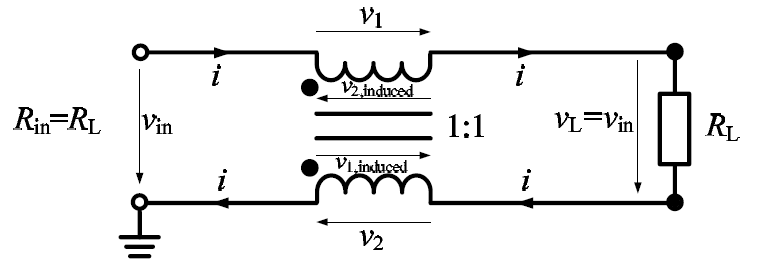
\includegraphics[width=8.5cm]{./bilder/components_current_balun.png}
    } \\
\parbox{9cm}{
    \textbf{Discrete LC Balun} \\
    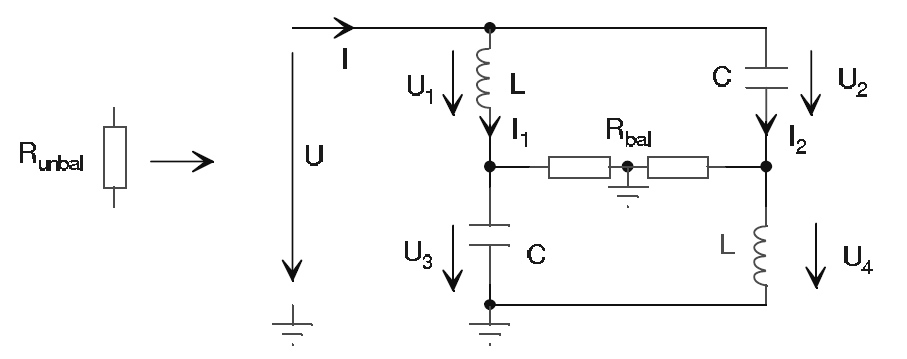
\includegraphics[width=8.5cm]{./bilder/components_discreteLC_balun.png} 
    }
& \parbox{9cm}{
    $ f_0 = \dfrac{1}{2 \pi \sqrt{LC}}$ \\
    $ C = \dfrac{1}{\omega \sqrt{R_{unbal} R_{bal}}} \qquad 
        L = \dfrac{\sqrt{R_{unbal} R_{bal}}}{\omega } $ \\ 
    $ R_{bal} = \dfrac{L}{R_{unbal} C}$    
        
        } \\
\end{tabular}

\newpage
\subsection{Mischer - Mixer \formelbuch{97}}
	Ein Mischer ist eine nichtlineare Komponenten, welche zwei Signale
    miteinander \textbf{multipliziert}. Es entstehen eine Summe und eine
    Differenz der beiden Eingangsfrequenzen. \\
    Somit kann ein Mischer ein Signal auf höhere Frequenzen rauf- oder auf
    tiefere Frequenzen runterkonvertieren. \\
    
\begin{tabular}{ll}
\parbox{9cm}{
    Folgende Ports stehen zur Verfügung:
    \begin{liste}
    	\item \textbf{RF} - Radio Frequency
    	\item \textbf{LO} - Local Oscillator
    	\item \textbf{IF} - Intermediate Frequency - Zwsichenfrequenz
    \end{liste}
    } & \parbox{9cm}{    
    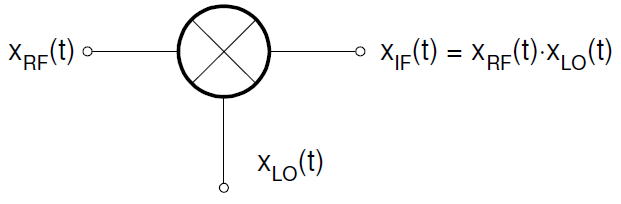
\includegraphics[width=7cm]{./bilder/components_mixer_schematic.png} } \\
\end{tabular}

\begin{tabular}{ll} 
\parbox{9cm}{
	\textbf{Aufwärtsmischen}    \\
	Die Zwischenfrequenz $f_{\text{IF}}$ wird auf die Frequenz des
	Lokaloszillators $f_{\text{LO}}$ raufkonvertiert. 
	Es entstehen links und rechts
	der Lokaloszillator-Frequenz jeweils zwei Spektren mit einem Abstand der Zwischenfrequenz. \\ \\
	
	\textbf{Abwärtsmischen} \\
	Hierbei wird die radio frequency $f_{\text{RF}}$ auf die Zwischenfrequenz 
	$f_{\text{IF}}$ runterkonvertiert.
	Es ist zu beachten, dass das RF Signal mit einem \textit{image rejection
	filter} versehen werden muss, sodass die sog. Spiegelfrequenz $f_{\text{image}}$ (image
	/ mirror frequency) gefiltert wird. Diese würde eine weitere Modulation
    auslösen und hätte eine Überlappung mit der Zwischenfrequenz
    $f_{\text{IF}}$ zur Folge.
    $$ f_{\text{RF}} = f_{LO} \pm f_{\text{IF}}  \quad
    \Longrightarrow \quad f_{\text{image}} = f_{LO} \mp f_{\text{IF}} $$ } &
    \parbox{9cm}{ 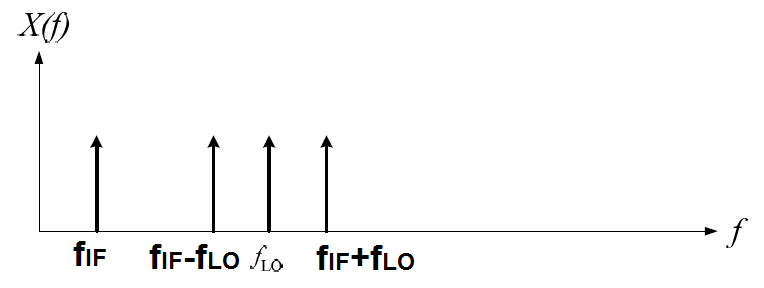
\includegraphics[width=9cm]{./bilder/components_mixer_spectrum.png} \\ \\
    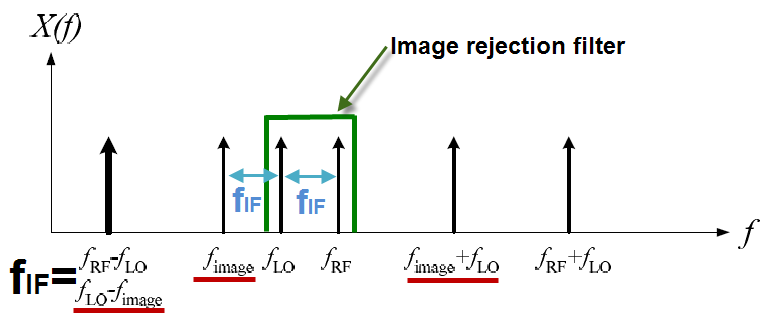
\includegraphics[width=9cm]{./bilder/components_mixer_image-frequency.png}}
    \\
\end{tabular}


\subsection{Oszillatoren \formelbuch{98}}

\begin{tabular}{lll} 
\parbox{9cm}{
	Wichtige Parameter von Oszillatoren:
	\begin{liste}
		\item Frequenzgenauigkeit (in ppm)
		\item Frequenzabweichung
		\item Einschwingzeit (bei Frequenänderung)
		\item Phasenrauschen
		\item Harmonische
	\end{liste} 
   
    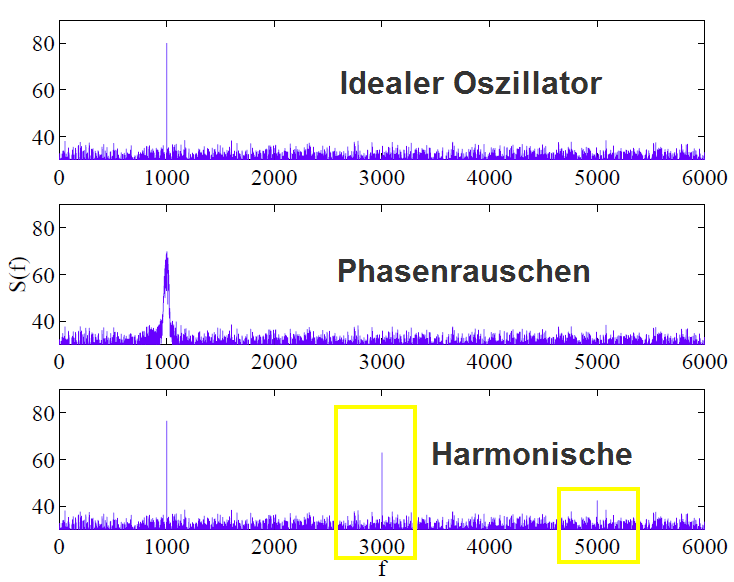
\includegraphics[width=9cm]{./bilder/components_oscillator_spectrum.png}} 

&	\parbox{5cm} {
	\textbf{Phasenrauschen}\\
	Nebst der Frequenzgenauigkeit ist das Phasenrauschen ein ebenso grosses
	Problem. Phasenrauschen sind \textbf{kurzzeitige zufällige
	Frequenzabweichungen}. \\
	Phasenrauschen wird als Leistungsdichte mit einseitigem Spektrum mit
	Frequenzabweichung $\Delta f$ im Bezug zur Trägerfrequenz angegeben.
	Die Steigung beträgt $-20$ dB/Dekade und stammt vom thermischen Rauschen der
	Verstärkerelementen im Oszillator.\\
	Das Phasenrauschen wird zum 1/f-Rauschen dazuaddiert, sodass das gesamte
	Spektrum resultiert. } & \parbox{4cm}{
    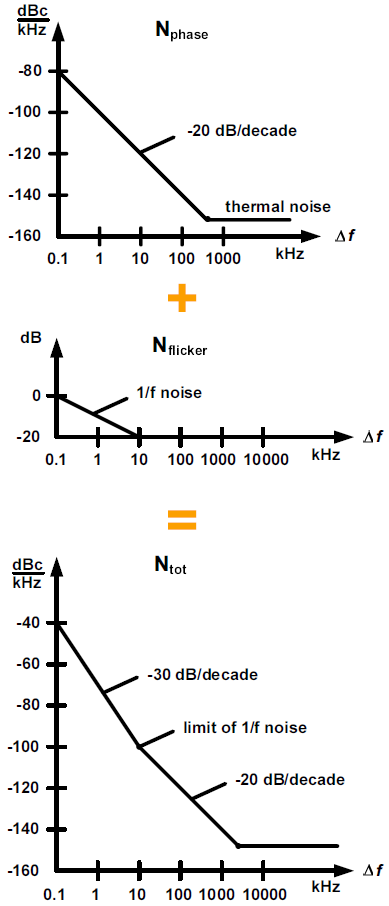
\includegraphics[width=4cm]{./bilder/components_oscillator_phase-noise.png}
    }
    \\
\end{tabular}

\newpage
\subsection{PLL und Synthesizer \formelbuch{100}}
Phase Locked Loops (PLL) können eingesetzt werden, um Frequenzen variabel zu
generieren oder Frequenzen zu vervielfachen. \\
Quarze mit tieferen Frequenzen (bspw.: 100MHz) haben bessere Genauigkeit
(kleiner ppm-Wert) als mit höheren Frequenzen (bspw.: 1GHz). Mit einem PLL kann
somit aus einem 100MHz Signal ein genaueres 1GHz Signal generiert werden. \\

\begin{tabular}{ll} 
\parbox{9cm}{
	\textbf{Integer-N Synthesizer} \\ 
	\includegraphics[width=9cm]{./bilder/components_pll_integerNsynthesizer.png}\\
	Phasenrauschen mit Faktor $N^2$ multipliziert am Ausgang \\
	Für grosse Auflösung: $f_r$ klein $\Rightarrow$ grosse Einschwingzeit}
& \parbox{9cm}{  
	\textbf{Fractional-N Synthesizer} \\
	\includegraphics[width=7.5cm]{./bilder/components_pll_fractorialNsynthesizer.png}\\
	\begin{liste}
      \item Frequenzteiler wird durch Counter umgeschaltet
      \item Frequenzauflösung feiner (nicht ganzzahlig) einstellbar
      \item Ausgangsfrequenz ändert über ein Zyklus, wenn Zeitkonstante von Loopfilter
        nicht genügend gross ist
    \end{liste}
    } \\
\parbox{9cm}{
    \textbf{Dual-Modulus Integer N Syntesizer}\\
    \includegraphics[width=7.5cm]{./bilder/components_pll_dual-modulus-integerNsynthesizer.png} \\
    $ T=(N+1)A+N(M-A) = A + MN $
    }
& \parbox{9cm}{
	\textbf{Direct digital synthesizer (DDS)} \\
	\includegraphics[width=7.5cm]{./bilder/components_pll_dds.png}\\
    \begin{liste}
      \item Bester Synthesizer für Phasenrauschen und Einschwingzeit.
      \item Frequenzeinstellung sehr flexibel
      \item Eher für tiefere Frequenzen (bis ca. 400 MHz)
    \end{liste}
	}
    \\
\end{tabular}

	

    
\subsection{HF-Filter \formelbuch{105}}
Für Hochfrequenztechnik sind folgende Filtertypen von Interesse: 
\begin{liste}
	\item Quarzkristall Filter
	\item Keramische Filter
	\item SAW (Surface Acoustic Wave) Filter
	\item Microstrip Filter (Transmission Line Filter)
	\item Passive LC-Filter, Aktive RC-Filter
\end{liste}

\subsubsection{Quarz Filter \formelbuch{105}}

\begin{tabular}{ll} 
\parbox{9cm}{
	\textbf{Quarz} \\ 
	\includegraphics[width=5cm]{./bilder/components_filter_quarz.png}	
	 } & \parbox{9cm}{  
	\textbf{Monolithischer Quarz} \\
	\includegraphics[width=7.5cm]{./bilder/components_filter_quarz-monolithic.png}\\
	Das Zweitor wird als Bandpassfilter genutzt \\
	Bandbreite $< 1\%$  zwischen $5 - 350$ MHz	
	}
\end{tabular}

\begin{tabular}{ll} 
\parbox{5.5cm}{
	\includegraphics[width=5.5cm]{./bilder/components_filter_rlc-resonator.png}	
	 } & \parbox{12cm}{ 
	\textbf{RLC-Schwingkreis}\\
		$$\omega_r=2\pi f_r=\dfrac 1{\sqrt{LC}} \qquad
		Q_{\text{ser}} =2\pi f_r \dfrac LR = \dfrac{\omega_r L}R \qquad
		Q_{\text{par}} = \dfrac R{\omega_r L} \qquad 
		W=\frac{2\Delta f}f= \frac 1Q $$ 
		$$\frac B{G+G_{\text{load}}} = \dfrac{1}{\frac 1{Q_0}+ \frac
		1{Q_{\text{ext}}}} = Q_{\text{loaded}} < Q_0 = \dfrac BG$$
		\underline{Seriell-/Parallelwandlung:}
		$$   R_p = R_s (1+Q^2) \qquad 
  L_p = L_s (1+\frac 1{Q^2}) \qquad 
  C_p = C_s (\frac{Q^2}{1+Q^2})$$ 
		
		 }
\end{tabular}

\subsubsection{Surface Acoustic Wafe (SAW) Filter \formelbuch{109}}
\begin{tabular}{lll} 
\parbox{6cm}{
	Bandpassfilter mit sehr hoher Güte $Q$\\
	Jedoch eher teuer \\
	Signal wird in akustisches Signal gewandelt, gefiltert \\ \\
	Ordnung des Filters beim Ablesen aus Network-Analyzer:\\ 
    $n = \frac{A_{1,dB}-A_{2,dB}}{20} \frac{1}{\log(\frac{f_2}{f_1})}$
	 } 
	 & \parbox{6cm}{ 	 
	\includegraphics[width=5.7cm]{./bilder/components_filter_SAW-schematic.png}	\\
	Typische Anpassschaltung		
		 }
	 & \parbox{6cm}{ 	 
	\includegraphics[width=5.7cm]{./bilder/components_filter_SAW.png}			
		 }
\end{tabular}

\subsubsection{Microstrip Filter \formelbuch{109}}
\begin{center}
	\includegraphics[width=10cm]{./bilder/components_filter_microstrip_types.png}
	\begin{tabular}{ll} 
\parbox{6cm}{
	\includegraphics[width=5.5cm]{./bilder/components_filter_microstrip_EM-field.png}	
		 } 
	& \parbox{6cm}{ 		
	$$  \varepsilon_{\text{eff}} \approx 
    \frac{\varepsilon_r+1}2+
    \frac{\varepsilon_r-1}2 \left(1+12\frac hw \right)^{-\frac 12}$$	
		 } 
\end{tabular}
	$$   Z_0 = \frac{60}{\sqrt{\varepsilon_{\text{eff}}}}
        \ln \left(8\frac hw+0.25\frac wh \right)\,[\Omega],
        \qquad w/h\le 1, \label{eq:line_impedance1} 
  \qquad Z_0 = \frac{120\pi / \sqrt{\varepsilon_{\text{eff}}}}%
         {w/h+1.393+0.667\ln (w/h+1.444)}\,[\Omega],
        \qquad w/h\ge 1  \label{eq:line_impedance2}$$	
\end{center} 	

\includegraphics[height=7cm]{./bilder/components_filter_microstrip_er.png}		
\includegraphics[height=7cm]{./bilder/components_filter_microstrip_ZL.png} \\

\begin{tabular}{|l|c|c|} \hline
                    & open         & short              \\ \hline \hline
 $l<\lambda/4$      & capacitive   & inductive          \\ \hline
 $l=\lambda/4$      & 0            &$\infty$            \\ 
                    & series resonance & parallel resonance \\ \hline
 $\lambda/4<l<\lambda/2$ & inductive   & capacitive    \\    \hline
 $l=\lambda/2$      &$\infty$          &0              \\
                    & parellel resonance & series resonance \\ \hline
 in general         &$ Z=-jZ_w\cdot \cot\left(\frac{2\pi l}{\lambda}\right)$
                    &$ Z=jZ_w\cdot \tan\left(\frac{2\pi l}{\lambda }\right)$\\
                    \hline
\end{tabular}
\begin{tabular}{|l|r|r|r|r|} \hline
PCB material & $\varepsilon_r$ & $\varepsilon_{\text{eff}}$
& $v/c$ & $Z_0$ \\ \hline \hline
Duroid                & 2.2 & 1.77 & 75\% & $94\,\Omega$ \\ \hline
epox-glass            & 4.8 & 3.4  & 54\% & $68\,\Omega$ \\ \hline
Alumina (Al$_2$O$_3$) & 9.8 & 6.5  & 39\% & $49\,\Omega$ \\ \hline
GaAs                  & 13  & 8.9  & 34\% & $43\,\Omega$ \\ \hline
Quartz (SiO$_2$)      & 3.8 & 2.89 & 58\% & $73\,\Omega$ \\ \hline
\end{tabular}

\begin{tabular}{ll} 
	\parbox{9cm}{
		\includegraphics[width=9.5cm]{./bilder/components_filter_microstrip_kuroda.png}	
	 } 
	 & \parbox{9cm}{ 	 
		\textbf{Designanleitung Microstripfilter}
		\begin{aufzaehlung}
        	\item Frequenzen des Analog-Designs mit Richards-Transformation
        	normieren: $\Omega =\tan\left(\dfrac{\pi f}{2f_0}\right)$
        	\item Filterkoeffizienten und dazugehörige Impedanzen berechnen. 
        	$ Z_i = \dfrac{g_{i-serie}}{\Omega'_c} \qquad Y_i =
        	\dfrac{g_{i-parallel}}{\Omega'_c}$
        	\item Nötige Bauelemente mit Kuroda Transformation (Abbildung links)
        	umformen, sodass zwischen jedem Element ein Einheitselement existiert.
        	\\
        	Normierte Impedanzen der resultierenden Elemente $Z_{i}$, sowie des
        	Einheitselements (Unit Element) $Z_{UEk}$ berechnen.
        	\item Impedanzen mit Systemimpedanz $Z_0$ entnormieren: $Z_{i}
        	\rightarrow Z_{ir}; Z_{UEk} \rightarrow Z_{UEkr}$
        	\item Verhältnis $w/h$ aller Impedanzen aus Grafik (oben rechts)
        	ablesen $\Rightarrow$ $w$ berechnen.
        	\item Effektive Dielektrizitätskonstante ($\varepsilon_{{\text{eff}}}$) aus Grafik
        	(oben links) ablesen und entsprechendes Wellenlängenverhältnis        
        	$\varepsilon_{{\text{eff}}}=\left(\frac{\lambda_0}{\lambda_m}\right)^2$ 
        	berechnen.
        	\item Länge der einzelnen Leitungselemente berechnen: \\
        	$l = \dfrac{c_m}{4 \cdot f_0} - \Delta l = 
        	\dfrac{c_0}{4 \cdot (\lambda_0 / \lambda_m) \cdot f_0} - \Delta l $ \\
        	$\Delta l = 0$ oder falls genau siehe Tabelle Praktikum 13.
        \end{aufzaehlung}		
	}
\end{tabular}
	


\subsection{Dioden \formelbuch{117}}
\subsubsection{Kapazitätsdiode - Varaktor \formelbuch{117}}
\begin{tabular}{ll} 
	\parbox{5cm}{
		\includegraphics[width=4cm]{./bilder/components_diode_varactor.png}	
	 } 
	& \parbox{13cm}{ 	 
		Kapazität abhängig von Spannung: $ C=C_0\left (1-\dfrac{U_b}{\Phi_b}
		\right )^{-n} \quad$
		Wird für VCO genutzt.
		}
\end{tabular}

\subsubsection{PIN Diode \formelbuch{117}}
Geeignet für Schalter bei HF-Anwendungen. 

\subsubsection{Schottky Diode \formelbuch{118}}
\begin{tabular}{ll} 
	\parbox{9cm}{
		\includegraphics[width=9cm]{./bilder/components_diode_schottky.png}	
	 } 
	& \parbox{9.5cm}{ 	 
		\begin{liste}
        	\item Kleinere Vorwärtsspannung ($ \approx 200 mV$) als gewöhnliche
        	Diode 
        	\item Schnelle Rückwärts-Erhohlzeit (Reverse Recovery Time)         
        \end{liste}
		}
\end{tabular}

\subsubsection{Tunneldiode \formelbuch{121}}
\begin{tabular}{ll}
    \parbox{4cm}{
        \includegraphics[width=3.5cm]{./bilder/components_diode_tunnel.png}
        }
    & \parbox{14cm}{
		Hat über einen gewissen Spannungsbereich einen negativen differentiellen
		Widerstand, was bei Oszillatoren zum Einsatz kommt.
        }
\end{tabular}


\section{Sender- / Empfängerarchitekturen \formelbuch{123}}
\newpage
\section{Übungs- und Praktikumsverzeichnis}
\renewcommand{\arraystretch}{0.85}
\begin{tabular}{|l|l|l|}
\hline
{\bf Beschreibung} & {\bf Praktikum} & {\bf Hausübung} \\
\hline
1dB Compression Point Beziehungen &            &       11.2 \\
\hline
     Aloha &            &        7.2 \\
\hline
Ausgangsimpedanz berechnen &        3.3 &            \\
\hline
Baluns in der Praxis &       12.1 &       12.2 \\
\hline
Baluns mit diskreten Elementen &       12.1 &            \\
\hline
Baluns mit Transformatoren &            &       12.1 \\
\hline
CDMA SNR vs. Carrier to Interference Ratio (C/I) &            &        7.4 \\
\hline
Dämpfer ausmessen &      2.1.4 &            \\
\hline
Dämpfer Pi-förmig & 2.1.2, 2.1.3 &            \\
\hline
Dämpfer T-förmig &      2.1.1 &        2.1 \\
\hline
   DCF-77  &          0 &        1.1 \\
\hline
Eingangsimpedanz berechnen &        3.3 &            \\
\hline
Excel Tabelle Noise Figure &         10 &            \\
\hline
Fehlerwahrscheinlichkeit - QPSK &        7.2 &            \\
\hline
Fragen Praktikums Themen &            &        5.5 \\
\hline
FSK Spektrum &        8.1 &        8.1 \\
\hline
   Funkuhr &          0 &        1.1 \\
\hline
GSM Kanäle &        5.1 &        7.1 \\
\hline
Güte bestimmen &            &        5.2 \\
\hline
$IIP_3$ bestimmen &            &       11.1 \\
\hline
$IIP_3$ Beziehungen  &            &       11.2 \\
\hline
Impedanzanpassung &            &   4.3, 5.3 \\
\hline
Kaskadierte $\frac{\lambda}{4}$ Transformatoren &        4.3 &            \\
\hline
Koaxialkabel Berechnungen &        4.1 &        4.2 \\
\hline
Korrelationsempfänger - MSK &        8.2 &            \\
\hline
Kuroda Transformation &            &     13.1.3 \\
\hline
Leistungsteiler &        2.2 &            \\
\hline
Leitungen  &        4.2 &        5.4 \\
\hline
Microstrip Bandpass Filter &            &       13.2 \\
\hline
Microstrip Tiefpass & 13.1, 13.2 &       13.1 \\
\hline
Mixer Parameter &       11.1 &            \\
\hline
Mixer Spektrale Messungen &       11.2 &            \\
\hline
MMIC Verstärker &        9.2 &            \\
\hline
Modulation &            &        8.2 \\
\hline
Monte Carlo Simulation &        7.1 &            \\
\hline
MSK - Korrelationsempfänger &        8.2 &            \\
\hline
Noise Figure einer Empfängerkette &         10 & 10.1, 11.1 \\
\hline
Noise Figure kaskadierter Verstärker &         10 &       10.2 \\
\hline
      OFDM &          6 &        6.1 \\
\hline
$OIP_3$ bestimmen &            &       11.1 \\
\hline
$OIP_3$ Beziehungen &            &       11.2 \\
\hline
optimale kapazitive Kopplung &        1.3 &        1.3 \\
\hline
Parasitäre Elemente &   1.2, 1.3 &        1.2 \\
\hline
QPSK - Fehlerwahrscheinlichkeit &        7.2 &            \\
\hline
SAW-Filter &        5.2 &            \\
\hline
SFDR bestimmen &            &       11.1 \\
\hline
Skin Effekt &            &        4.1 \\
\hline
Smith Chart Admittanzen einzeichnen &            &        2.3 \\
\hline
Smith Chart Eingangsimpedanz bestimmen mit Impedanz und Admittanz Chart &            &        3.1 \\
\hline
Smith Chart geometrische Orte einzeichnen  &            &        3.2 \\
\hline
Smith Chart konstante Güte &            &        5.2 \\
\hline
Smith Chart Leitungen transofmieren &            & 5.4.3, 5.4.4 \\
\hline
Smith Chart mit MatLab &        3.1 &            \\
\hline
Smith Chart Punkte konstruieren &            &        2.2 \\
\hline
Smith Chart VSWR Kreise &            &        2.4 \\
\hline
Spannungs-Stehwellenmuster &            &      5.4.2 \\
\hline
Spektrum nichtlinerare Komponenten &        5.3 &            \\
\hline
Stabilität Verstärker &        9.1 &            \\
\hline
TDMA Effizienz &            &        7.3 \\
\hline
Verluste bei Fehlanpassung &        3.2 &        3.3 \\
\hline
Verstärker MMIC &        9.2 &            \\
\hline
Verstärker S-Parameter &            &        9.1 \\
\hline
Verstärker Stabilität &        9.1 &            \\
\hline
\end{tabular}  
\renewcommand{\arraystretch}{1}

\end{document}
